% ============================================================================
% Overleaf 主文件(GB/T 7714-2015 数字顺序制)
% 编译:XeLaTeX -> BibTeX -> XeLaTeX -> XeLaTeX
% ============================================================================
\documentclass[fontset=fandol,12pt,a4paper,oneside]{ctexbook}
\usepackage{geometry}
\geometry{left=3cm,right=2.5cm,top=2.5cm,bottom=2.5cm}
\usepackage{graphicx}
\usepackage{booktabs,threeparttable}
\usepackage{amsmath,amssymb}
\usepackage{bm}
\usepackage{natbib}
\usepackage{hyperref}
\hypersetup{colorlinks=true,linkcolor=black,citecolor=blue,urlcolor=blue}

% 术语宏
\newcommand{\II}{\textit{II}}

% 参考文献样式(GB/T 7714-2015)
% 可选:gbt7714-numerical 或 gbt7714-author-year
\bibliographystyle{gbt7714-numerical}

\begin{document}
\setcounter{tocdepth}{2}
\tableofcontents
\listoffigures
\listoftables
% ==========================
% 缩略语表(可选,但常用)
% ==========================
\chapter*{缩略语表}
\begin{tabular}{lp{10cm}}
DID & Difference-in-Differences,双重差分 \\
ATT & Average Treatment Effect on the Treated,处理组平均处理效应 \\
FE & Fixed Effects,固定效应 \\
II & Industry Influence Intensity,方向性行业影响强度 \\
SUTVA & Stable Unit Treatment Value Assumption,稳定单元处理值假设 \\
TVP-VAR & Time-Varying Parameter VAR,时变参数向量自回归 \\
\end{tabular}


% 章节(从 子目录“final_tex/” 引入)
% 注意:为避免 Overleaf 在子目录写 .aux 的权限/编码问题,这里改用 \input
% ==========================
% 前置:摘要与关键词(中文/英文)
% ==========================
\chapter*{摘 要}
基于2010—2018年40个行业、1{,}599个行业配对的月度面板数据,本文在链路(行业配对)层面识别供给侧结构性去产能政策对跨行业风险溢出的影响。研究采用双重差分(DID)与事件研究相结合的统一框架,以方向性行业影响强度(II)为因变量,设置配对固定效应与时间固定效应,并在配对层进行聚类稳健推断。在平均效应层面,处理组行业相对对照组的II显著下降,表明政策对跨行业风险外溢具有相对抑制作用;在动态层面,政策实施当年效应不显著,随后逐步显现并持续存在,符合“价格—数量—信用”三通道的传导时滞;在结构性层面,基于“政策前对处理邻居的预暴露”的分组显示,高预暴露链路在政策后的抑制更强,提供了“产业链稳定器”(议价、信息、协同)机制的结构化证据。两类稳健性检验(控制变量扩展与缩尾敏感性)表明主结论在合理口径下保持稳健。

本文的贡献在于:第一,将“方向性—链路级”度量与因果识别耦合,避免宏观联动与共同趋势被误判为政策效应;第二,以政策前“预暴露”构造结构性剂量并刻画“剂量—响应”,揭示何处抑制更强并为链路治理提供依据;第三,将识别证据转译为政策工具,提出“稳链优先序—协同披露—压力测试分层”的可操作建议。研究为评估结构性产业政策在网络中的作用提供了方法参考,亦为“去产能—稳链—高质量增长”的政策组合提供证据支持。

\vspace{0.5em}
\noindent\textbf{关键词:} 去产能;行业风险溢出;双重差分;事件研究;生产网络;结构性异质性

\chapter*{Abstract}
Using monthly panel data of 40 industries and 1,599 directed industry pairs from 2010 to 2018, this study identifies the impact of China’s supply‐side capacity reduction policy on inter‐industry risk spillovers at the link (pair) level. We employ a unified framework combining Difference‐in‐Differences (DID) with an event‐study design, using the directional industry influence intensity (II) as the outcome, with pair and time fixed effects and cluster‐robust inference at the pair level. On average, the II of treated industries declines relative to controls, indicating a policy‐induced attenuation of cross‐industry spillovers. Dynamically, the effect is insignificant in the implementation year, then emerges and persists, consistent with frictions along price–quantity–credit channels. Structurally, pre‐policy exposure to treated neighbors exhibits a dose–response pattern: links with higher pre‐exposure display stronger post‐policy attenuation, consistent with a “supply‐chain stabilizer” mechanism (bargaining, information, coordination). Robustness checks on control expansion and winsorization confirm the stability of the main findings.

This paper contributes by: (i) integrating directional, link‐level measures with causal identification to avoid confounding macro comovements with policy effects; (ii) introducing pre‐policy exposure as a structural dose to reveal where attenuation is stronger and to inform link‐level governance; and (iii) translating evidence into actionable policy tools—prioritized link stabilization, coordinated disclosure, and exposure‐tiered stress testing. The results offer methodological guidance for evaluating structural industrial policies in networked settings and provide evidence for the “capacity reduction–stable chains–high‐quality growth” policy mix.

\vspace{0.5em}
\noindent\textbf{Keywords:} capacity reduction; inter‐industry spillovers; DID; event study; production networks; structural heterogeneity

% ============================================================================
% 第1章 绪论(按项目大纲,仅二级目录:1.1/1.2/1.3)
% ============================================================================
\chapter{绪论}
\label{chap:intro}

\section{研究背景与意义}
2014年起,去产能政策在钢铁、煤炭、建材与部分高能耗制造业持续推进,客观上重塑受影响行业(处理组)的成本结构与资产负债表,并可能通过上下游交易、信用约束与共同预期触发跨行业风险联动。若停留在行业或宏观均值层面,既难以回答“谁影响谁、何时影响、影响几何”,也难以剥离共同趋势与结构性净效应。因而需要在网络情境下,以可识别的因果框架刻画政策对跨行业风险溢出的相对净影响。

网络视角的必要性体现在三点:
\begin{enumerate}
  \item 级联与非对称:上游供给冲击沿“价格—数量—库存约束”传导,下游需求收缩反向影响投资与现金流,方向性显著;
  \item 度量语义:行业间“向外/向内/净效应”并不对称,无向相关易掩盖“谁影响谁”的本质;
  \item 融资与预期共振:金融约束与市场预期与实物流共同作用,使“同向共振—异向抵消—局部瓶颈”并存,需在“有向、随时间变化”的框架下识别路径与强度。
\end{enumerate}

本文采用“公司层格兰杰显著性→行业配对归一化”的方向性强度指标,记为 \II(取值归一化至 [0,1]),以“链路/配对($i\to j$)”为单位进入 DID 框架识别政策的\emph{相对净效应}。并将政策前窗口(2010—2013 年)中行业与“处理邻居”的结构性耦合强度定义为“预暴露”,用于刻画\emph{结构性异质性}:链路越紧密,越可能内生形成“议价—信息—协同”的稳定器,由此在政策后表现为更明显的抑制效应。

理论意义在于:在网络情境下提供方向性溢出的因果识别,将连通性/生产网络与 DID/事件研究耦合;将“预暴露”作为结构性剂量纳入链路层分析,补足“行业/公司”层之外的证据。现实意义在于:把“稳链—补链—强链”的宏观目标转译为可操作的\emph{链路治理}工具,包括\emph{前置校准}(将预暴露纳入监测清单)、\emph{差异化缓冲}(账期协调、阶段性价格稳定、联合采购与信用支持)与\emph{协同信息披露}(跨部门与链路的信息共享),减少“同质化扩张—价格战—再过剩”的内卷回路。



\section{研究内容和技术路线}
本文围绕三项可检验问题:
\begin{enumerate}
  \item 平均效应:去产能实施后,处理组相对对照组的 \II 是否下降?若 DID 交互项系数 $\beta<0$,则为相对抑制;
  \item 动态与识别:政策前是否满足平行趋势?政策效应沿时间如何演进(事件研究)?
  \item 结构性异质性:预暴露是否呈现“剂量—响应”,即高预暴露链路抑制更强?
\end{enumerate}

技术路线遵循“事实—识别—机制—稳健”。第一,事实:在政策前后窗口构建行业配对的风险溢出网络,报告方向性强度与结构特征;第二,识别:在统一口径下实施 DID 与事件研究,设置配对固定效应与时间固定效应,标准误在配对层聚类,确保相对净效应与动态路径的可解释性;第三,机制/结构:以“预暴露”刻画结构性异质性,采用分组或交互识别“剂量—响应”;第四,稳健:在缩尾、滞后、样本窗口与安慰剂等维度进行系统检验。

数据与口径声明(与第\ref{chapter:data_method}章一致):样本窗口 2010—2018 年(月度),行业口径 40 个,形成 1,599 个有向行业配对,共 148\,050 个“配对—月份”。政策时点 2014-01。主结果采用滞后 $=3$ 与 $5~\%$ 缩尾;其余滞后与缩尾口径仅作稳健性对照。变量构造:\II 反映当期方向性强度,由公司层格兰杰显著性占比汇聚并归一化得到。预暴露刻画政策前窗口对处理邻居的结构性耦合强度,仅用于分组与展示;控制变量在发送与接收两侧对称纳入(资产负债率、ROA、TobinQ),以减少遗漏异质性的风险。



\section{创新之处}
\begin{enumerate}
  \item 识别:在网络图的绝对对比之外,提供方向性 \II 的 DID/事件研究因果估计,避免共同时间趋势被误判为政策效应;
  \item 结构:以“对处理邻居预暴露”作为链路层结构剂量,验证“剂量—响应”,补足行业/公司层之外的结构性证据;
  \item 机制:提出“议价—信息—协同”的稳定器机制,并与链路治理工具对接(稳链优先序、协同披露、分层压力测试)。
\end{enumerate}

局限与边界(不影响主结论):(1)口径依赖——主结果使用滞后 $=3$ 与 $5~\%$ 缩尾,其他设定仅作稳健性对照;(2)机制变量的直接可观测性有限——价格/账期/信用链条等“软变量”在数据可得时可作为后续扩展;(3)统一政策时点便于识别平均效应,但分行业/分地区节奏的细目刻画仍有拓展空间。

% ============================================================================
% 第2章 文献综述(仅使用二级目录,不新增更深层级)
% ============================================================================
\chapter{文献综述及理论基础}
\label{chap:literature}

\section{概念界定}
为避免口径混淆,本文对核心概念做统一界定:
\begin{enumerate}
  \item 行业影响强度(\II):基于公司层格兰杰有向预测关系,按行业聚合得到“$i\to j$”在期 $t$ 的方向性强度,归一化至 $[0,1]$,用于进入 DID/事件研究识别相对净效应;
  \item 预暴露(Exposure):在政策前窗口(2010—2013年)对“处理邻居”的耦合强度聚合(如两端最大值/均值),作为结构性剂量用于异质性分组或交互;
  \item 识别框架:双重差分(DID)刻画平均处理效应,事件研究检验平行趋势与动态路径;固定效应设置为配对($i,j$)与时间($t$),标准误在配对层聚类。
\end{enumerate}

\section{文献综述(结构化)}
围绕“怎么量—为什么传—怎么识别”的主线,现有研究可分为三条相互补充的谱系:
\begin{enumerate}
  \item 溢出度量与网络连通性:从单资产流动性到系统连通性,度量从无向相关拓展到有向网络与方差分解,强调“向外/向内/净溢出”的区分与多层归因\citep{billio2012econometric,diebold2012better,diebold2014connectedness}。本文不并行采用 VAR‑FEVD/TVP‑VAR/频域口径,而是选择可直接进入因果识别的链路级方向性指标(\II)。
  \item 生产网络与跨行业传播:微观冲击沿投入—产出关系传播,选择性放大形成宏观波动\citep{acemoglu2012network,carvalho2014micro}。中国背景下,关键行业与周期位置共同决定传播方向与强度,存在非对称的“向外/向内”能力。本文据此在链路层刻画方向性与结构异质性。
  \item 政策评估与识别设计:DID/事件研究在处理异期效应与平行趋势时需谨慎设置固定效应与聚类推断\citep{sun2021event,bertrand2004much,cameron2015practitioner,angrist2009mostly}。本文采用统一口径(配对FE+时间FE、配对聚类SE)并以矩阵式稳健性(缩尾、滞后、窗口、安慰剂)验证结论稳定性。
\end{enumerate}

\section{理论基础}
围绕“方向性—动态—识别”三条主线,本文采用与经验证据紧密相连的理论支撑:
\begin{enumerate}
  \item 生产网络的方向性与选择性放大:投入—产出网络中,节点位置(上/下游)、路径长度与耦合强度决定冲击的方向性与选择性放大\citep{acemoglu2012network,carvalho2014micro}。当共同时间冲击被吸收后,链路级的相对变化(处理组相对对照组)可体现为“相对抑制”($\beta<0$),与网络乘数的差异化传导相一致;
  \item 动态调整与时滞的经验事实:合同刚性、库存与账期等摩擦常导致“政策当年效应不显著—次年起显现—随后持续/收敛”的时间结构。这种时滞属于经验层面的动态特征,解释了事件研究路径的形状,但不被上升为独立的理论门派;
  \item 网络情境下的因果识别与干扰:在异期处理与组间异质性存在时,DID/事件研究需要避免系数污染,采用恰当的固定效应与聚类推断\citep{sun2021event,bertrand2004much,cameron2015practitioner,angrist2009mostly};在一般干扰(interference)不可完全排除的网络环境下,可通过固定结构性剂量(预暴露)进行分组/交互检验,并辅以安慰剂与口径敏感性以验证稳健性\citep{aronow2017interference,athey2018network}。
\end{enumerate}

\section{流动性与溢出测度}
度量“谁影响谁、影响有多强以及方向为何”的首要问题,是建立具有解释力与可复现实证口径的溢出(connectedness)或联动(spillover)指标。早期以流动性为核心的研究(如Amihud测度)强调单资产随时间的摩擦与补偿关系,但难以揭示主体间有向作用。连通性框架的兴起(如\citep{billio2012econometric,diebold2012better,diebold2014connectedness})将方差分解与网络表示结合,把“来自他人的解释份额”解释为“被他人影响的强度”,并进一步区分“向外/向内/净溢出”。这一谱系的优势在于:一是提供了“系统—子系统—主体”多层的归因;二是天然适配图结构,使“方向性”与“重要边”可以被识别。然而,其方法实现面临三个常见抉择:窗口滚动 vs. 时变参数(TVP)、时域 vs. 频域、参数稳健性 vs. 解释力。

就方法定位而言,本文不并行采用 VAR‑FEVD、TVP‑VAR 或频域连通性等系统级度量;相关方法仅作为文献对话中的背景与参照,用以说明不同口径的优劣取舍与适用场景,避免读者误解为本文所使用的识别与度量口径。

基于上述权衡,本文采取“公司层格兰杰显著性→行业配对归一化”的方向性强度度量(II):先在公司层识别显著的有向预测关系,再按行业聚合为“i→j”在当期的显著性占比,并归一化到[0,1]。这一口径有三点考虑:(1)链路粒度:面向“配对(pair)/链路”而非“行业整体”,可以直接进入双重差分(DID)识别相对净效应;(2)方向语义:II天然表达“谁到谁”的当期方向性,避免无向相关性掩盖非对称传播;(3)稳健性矩阵:II对滞后阶、阈值与极端值处理敏感,需配套“滞后(lag=1/2/3)、缩尾(none/1/5/10%)、窗口(去极端年)、安慰剂(虚假时点/组)”等矩阵化稳健性。与此同时,我们承认FEVD/TVP‑VAR/频域等方法在描述“系统级—周期段”的解释力,因而在文献对话中对其优缺点进行“可替代但不冗余”的定位:II强调“链路级—当期—可入DID”的可识别性,系统级刻画可以作为补充,但不宜在本文中与主识别口径并行,以免产生口径杂糅与推断混淆。

方法学上,“方向性—有向网络”是连通性框架区别于一般协方差或相关系数的根本所在。Diebold–Yılmaz的方差分解、Baruník–Křehlík的频域分解与TVP‑VAR等方法各有侧重,但在本文中均不作为实证口径使用,仅作背景参照。本文从识别设计出发,将 II 作为“进入因果识别”的主口径:一方面在图结构上具备“边”的含义,另一方面在估计上可以与事件研究、DID与预趋势检验无缝衔接。当核心命题从“是否存在联动”转向“政策如何改变联动”时,度量的可识别性优先于系统层全面性,II 作为主口径更契合本文的目标函数。

\noindent\textit{与本研究假设的对应关系}:本节的方法讨论支撑 H1(平均效应)的可检验性——方向性 II 能以链路(i→j)为单位进入 DID/事件研究,从而识别“相对抑制”的符号与幅度;同时为 H2(结构性异质性)提供方向性语义与度量基础(预暴露按“对处理邻居”的方向性聚合),并为后文的政策启示留出工具化空间。
\section{行业间风险传染与产业链结构}
生产网络文献强调:微观冲击如何沿投入—产出关系传播,并在某些节点被放大,最终形成宏观层面的波动\citep{acemoglu2012network,carvalho2014micro}。在这一框架下,“节点—边—路径—团簇”的组合结构决定了传播的幅度与方向性;若把行业视为节点、交易视为边,则上游供给约束与下游需求收缩会沿既有链路累积,形成“瓶颈—溢出—放大”的链式逻辑。中国背景下的实证证据显示:主导行业随发展阶段而变迁,建筑/房地产常扮演“传导—放大”的关键角色,网络结构与周期位置共同决定冲击的宏观显化\citep{huang2024network}。同时,行业的“上行/下行风险”并不对称——金融主导的上行情绪可能局部提升“向外”强度,而实体部门在下行期的库存/订单约束会更快地压缩“向内”接收能力\citep{lizheng2024updown}。这些事实共同提示:仅在行业总体层面比较均值,容易忽略“谁影响谁”的非对称性;仅在宏观层面观察波动,也难以对链路级别的治理提出具体工具。

与生产网络并行,金融联动与市场预期也在“放大—吸收”的过程中发生作用:价格、数量与信用约束的三通道会出现阶段性“共振”或“抵消”,冲击在某些链路可能被扩张融资或合同协同所“吸收”;而在另一部分链路,则因融资边际收缩与信息不对称被显著加强。把这三通道纳入解释框架,一方面有助于识别“政策当年效应可能不显著—随后显现”的时滞结构,另一方面也提醒我们在因果识别中严谨控制共同时间冲击,避免把“共振”误判为“政策”。

本文采取“链路(pair)层”的视角,直接在“i→j”的方向上检验政策影响强度的相对净效应,避免行业整体层可能掩盖的非对称传播;同时,以“政策前对处理邻居的预暴露”刻画结构性耦合强度,识别“冲击更易传到哪里、在哪些链路更可能被吸收”的异质性。在此过程中,“事实—识别—机制”的分层叙事尤为重要:事实层面,政策前后网络结构是否发生可观测变化;识别层面,DID/事件研究是否支持“相对抑制”的因果陈述;机制层面,结构性耦合是否解释“抑制更强”的剂量—响应。

\noindent\textit{与本研究假设的对应关系}:本节的生产网络与传播逻辑为 H2(结构性异质性)提供理论支撑:预暴露越高,沿链路的耦合越强,越可能在政策后呈现“更强抑制”的剂量—响应;同时也为 H1(方向性联动的“相对抑制”)提供了“为何可能”的结构直觉。
\section{政策评估的识别方法}
双重差分(DID)在政策评估中的长处在于:通过处理组与对照组在政策前后变动的差异,识别“相对净效应”,从而部分剔除共同趋势。但在分期施治与组间异质性广泛存在时,传统TWFE(双向固定效应)框架的“组—时”系数可能被异期效应污染,导致预趋势检验出现“伪显著”或政策后效应被低估/夸大\citep{sun2021event}。因此,本文在设计上把“基准DID+事件研究”作为识别主干:前者提供“平均处理效应(ATT)”的估计,后者用“相对期(k)”的路径系数检验平行趋势与时滞结构。从固定效应角度,我们在配对(pair)层设置个体固定效应控制不随时间变化的“链路异质性”,在时间层设置共同时间效应以吸收宏观冲击;标准误在配对层聚类,处理同一配对的序列相关与组内相关\citep{bertrand2004much,cameron2015practitioner}。

识别假设的操作化包括三点:其一,平行趋势——用事件研究在政策前窗口检验各相对期系数是否显著偏离0;其二,无共时重大政策干扰——在口径声明与稳健性设计中增加对潜在干扰年份/事件的处理(例如去极端年或替代窗口);其三,一般干扰(interference)——在网络环境下,链路间可能存在相互影响,本文通过在分组内固定“政策前预暴露”并作为结构性剂量进行异质性识别,减少链路间交叉溢出对“平均效应”的污染,并在稳健性中扫描阈值、聚合与方向口径以验证稳健结论\citep{aronow2017interference,athey2018network}。此外,为缓解口径敏感性,我们采用“缩尾—滞后—窗口—安慰剂”四维矩阵:缩尾处理(none/1/5/10%)抑制极端值的驱动效应;滞后(lag=1/2/3)验证II构造与预测结构的鲁棒性;窗口(例如剔除特殊年份)检验样本敏感性;安慰剂(虚假时点/虚假处理组)检验模型在“无政策”条件下的虚假显著概率。

\noindent\textit{与本研究假设的对应关系}:本节识别框架直接服务于 H1——DID估计量与事件研究的路径系数分别刻画“相对净效应”和“动态演化/平行趋势”;同时提供 H2 的实施语法(预暴露×Post 或分组 DID/事件对比)以验证“剂量—响应”。
在“度量—结构—识别”的框架中,DID/事件研究回答“政策有没有改变联动、方向与平均幅度如何”;而要解释“哪里更抑制/更显著”,需要引入结构性剂量维度。下一节我们讨论“预暴露”作为结构剂量的设计逻辑与机制含义。

\section{产业链结构与稳定器机制}
“预暴露(exposure)”指政策前窗口内,行业相对于“处理行业集合”的结构性耦合强度。本文采用“向处理邻居的II强度聚合(如两端max)”作为链路层的结构剂量,用于异质性分组或交互,不作为工具变量以避免Bartik类识别争议\citep{goldsmithpinkham2020bartik}。其经济含义在于:预暴露越高,链路越紧密,越可能存在内生的“协同—分担—缓冲”安排,从而在政策后出现“II下降更显著”的抑制现象。

稳定器机制可以从三条渠道解释:第一,议价与合同协同——处理邻居在冲击期更倾向于协调账期、阶段性锁价、共同分担边际成本,通过“合同—信用—供货节奏”的组合协商来内部化短期冲击;第二,信息优势与联合排产——紧密链路更早共享供需与库存信息,形成“联合排产/备货—柔性产能—库存协同”,降低预测误差与被动减产所致的外溢;第三,共享资源与信用支持——在关键时点形成“联合采购与授信背书”安排,以抵消下游需求或上游供给的阶段性波动。三者共同作用,使高预暴露链路在政策后呈现更强的“相对抑制”,而低预暴露链路则更易体现“市场化传导”的直接外溢。

从设计角度,预暴露的阈值(分位数切分)、聚合(max/mean)与方向(out/in/total)口径会影响“组内混合度—噪声”之间的平衡。经验上,为兼顾异质性识别与预检(平行趋势)的稳定性,可取顶/底分位(例如q=0.30)进行“高/低暴露”分组,并丢弃中间样本以提高组内同质性;同时在附录报出敏感性扫描,展示在不同阈值与聚合口径下结论方向一致。需要强调的是:预暴露属于“结构性描述量”,目标是帮助解释“在哪里更抑制”,而非作为外生工具直接识别因果;因此,我们把它限定在“分组/交互—剂量—响应”的语法中与DID/事件研究配合使用。

\noindent\textit{与本研究假设的对应关系}:本节机制阐释与口径设计正对应 H2:若高预暴露链路在政策后更易通过议价/信息/协同内生出缓冲机制,则应观察到“高暴露组的DID更负/事件路径更向下”;该结构性证据亦可转化为“链路治理”的政策启示依据(不作为本文的可检验假设)。
\section{文献述评与研究空白}
综合上述脉络,可以把现有研究的“位势图”概括为三种偏好:一类聚焦“系统层的联动事实”,在连通性与网络拓扑上给出丰富描述,但对“为什么变化、政策如何改变联动”的因果阐释不足;一类聚焦“政策评估的平均处理效应”,在个体/行业层进行DID识别,但缺乏在网络情境下的方向性刻画与结构维度;还有一类使用“节点属性(强度/位置)”解释结构差异,但在“哪里更抑制”的问题上缺少可度量、可操作的剂量维度。相较之下,本文在三方面补位:(1)在网络情境下以“方向性II”进入DID与事件研究,识别“相对净效应”,避免将共同趋势误判为政策;(2)以“政策前对处理邻居的预暴露”作为结构性\emph{剂量},从“更强—更弱”的梯度关系来解释“哪里更抑制”,并通过阈值/聚合敏感性扫描降低经验性参数依赖;(3)在稳健性矩阵上对“缩尾—滞后—窗口—安慰剂”进行系统化覆盖,提高因果陈述的稳健程度。

在中国语境下,“去产能—稳链—反内卷”提供了一个将证据转译为治理工具的应用场景:本文的结构化识别为“链路治理”提供三条可操作路径——关键链路的\emph{前置校准}(早识别、早介入)、\emph{差异化缓冲}(账期/锁价/联合采购/信用支持)与\emph{协同披露}(跨部门与链路的信息同步)。这类工具并不依赖于某一行业或某一模型,而源自“方向性—结构剂量—相对净效应”的方法学闭环,具有跨行业的可迁移性。

\noindent\textit{与本研究假设的对应关系}:本节综述把文献位势图与本文三大假设对齐:H1——在方向性度量与DID/事件研究框架下识别“相对抑制”;H2——以“政策前对处理邻居的预暴露”刻画结构剂量并验证“剂量—响应”;并据此将 H1+H2 的经验证据转译为“链路治理”的可操作工具(前置校准、差异化缓冲、协同披露),作为本文的政策启示(非可检验假设)。
\section{小结}
本章从“怎么量—为什么传—怎么识别因果—结构剂量与机制—中国式治理语境”的主线出发,对相关文献与方法做了结构化梳理。首先,连通性/溢出度量为方向性与强度提供了可计算口径;在此基础上,生产网络与金融联动的理论与证据说明了冲击沿链路传播的条件与方向。其次,DID与事件研究在“相对净效应—动态路径—预趋势检验”的框架下,为政策评估提供了可操作识别;针对网络中的一般干扰,本文将“政策前对处理邻居的预暴露”设计为结构性剂量以刻画异质性,并通过敏感性扫描增强稳健性。最后,在中国“去产能—稳链—反内卷”的语境下,本文把“相对抑制+预暴露梯度”的证据转译为三类链路治理工具。下一章(第\ref{chap:theory}章)据此提出可检验假说,并在第\ref{chapter:data_method}章给出数据、变量与模型设定;第\ref{chap:empirical}章呈现基准DID、事件研究与基于预暴露的异质性结果;第\ref{chap:conclusion}章总结研究结论并讨论政策建议。
% ============================================================================
% 第3章 理论与研究设计(仅使用二级目录,不新增更深层级)
% ============================================================================
\chapter{理论与研究设计}
\label{chap:theory}

\section{理论框架}
去产能政策通过价格、数量与融资约束三条通道改变受影响行业的行为边界,并沿既有的投入—产出与合同—信用关系向外传导。上游行业的供给侧收缩,首先在价格与交付周期上体现为对下游的成本与库存压力,随后通过订单节奏、联合排产、存货周转与现金流安排反馈到下游产出决策;反向地,下游需求的收敛也会通过数量与预期渠道压缩上游投资、产能利用与经营性现金流。在这一“实物流—信息—信用”交织的网络中,政策冲击很少即刻、对称地体现在所有链路上,而是呈现出“方向性、阶段性与选择性”三种特征。

方向性在于,行业配对(i→j)所承载的经济含义并不等同于(j→i):前者对应发送行业对接收行业的当期影响强度,后者则反映反向约束或需求侧反馈。若使用行业整体均值或无向相关,容易掩盖“谁影响谁”的真实结构,从而在政策评估中把“共同趋势”误判为“净效应”。阶段性在于,合同、库存与账期等摩擦普遍存在,政策当年的可观测效应常常并不显著,待到价格—数量—信用三通道逐步完成“再均衡”后,政策影响才在次年及其后持续显现。选择性在于,并非所有链路都以同样力度响应:对“处理邻居”的耦合强度更高的链路,可能在政策后体现出更强的抑制,这既与传播路径长度、耦合强度与议价结构相关,也与链路上“信息与协同”的可行性相关。

为刻画上述结构差异,本文在行业配对层使用方向性强度指标(II)作为被解释变量:II 由公司层面的有向预测关系汇聚而来,归一化后反映当期 i→j 的影响强度;并在政策前窗口构造“对处理邻居的预暴露”,用于识别“哪里更易被冲击、哪里更可能吸收冲击”的结构性异质性。直观地讲,预暴露越高,链路越紧密,越可能在冲击发生时依靠“议价—信息—协同”三类安排内生出缓冲机制:通过账期协调、阶段性价格稳定与成本分摊、联合排产与库存协同、联合采购与共享信用支持等工具,降低短期外溢并把冲击的一部分“消化”在链路内部。这一机制在“相对净效应”的框架下,表现为政策后 II 的相对下降更为明显。

上述框架在经验上导向两个可检验的命题:第一,处理组行业相对对照组的方向性强度 II 在政策后呈“相对抑制”(平均效应);第二,政策前对处理邻居的预暴露越高,政策后 II 的相对下降越明显(结构性异质性)。二者共同构成本文“方向性—因果识别—结构剂量”的识别主线。值得强调的是,本文的目标并非描述绝对的前后变化,而是在控制共同时间冲击与链路不变异质性的前提下,识别“政策如何改变联动”。

\section{研究假设}
基于上述理论框架,本文提出以下两个可检验假设,并明确其统计含义与验证路径:

\noindent\textbf{H1(平均效应:相对抑制)}:政策实施后,处理组行业相对对照组的方向性强度(II)增幅更小或出现下降,即“相对抑制”成立。

\noindent\textit{验证路径}:在行业配对层估计双重差分模型,设置配对固定效应与时间固定效应,并在配对层聚类稳健标准误。若交互项系数为负且显著,则表明政策对跨行业传播的相对抑制成立。为检验识别假设,采用事件研究在政策前窗口观察各相对期系数是否围绕零波动;在政策后窗口,系数应在合理的时滞后逐步显现并保持方向一致。若交互项不显著或为正,则需复核平行趋势、潜在共时干扰与口径设定,谨慎解释“无明显相对抑制”的可能性。

\noindent\textbf{H2(结构性异质性:剂量—响应)}:政策前对处理邻居预暴露越高的链路,政策后的相对抑制越强。

\noindent\textit{验证路径}:将样本按政策前预暴露的顶/底分位划分为“高/低暴露组”,分别在子样本上估计双重差分模型;若高暴露组的交互项估计值更为负向(且显著),则支持“剂量—响应”的结构性异质性。亦可通过在全样本中加入“预暴露×政策后”或“预暴露×处理×政策后”的交互项,检验交互系数是否显著为负。为保证分组内识别的有效性,应在政策前窗口对各组的相对期系数进行预检,并以阈值/聚合口径的敏感性扫描验证方向稳定性。若异质性证据不显著,可能源于阈值设置过于极端导致组内混合不足,或结构性梯度本身并不强,需要在稳健性中进一步检验。

上述两个假设共同回答“有没有相对抑制”与“在哪些链路更强”。它们面向经验上的可验证问题,均可通过双重差分与事件研究的常见语法落地。至于治理上的含义——例如将“预暴露”纳入前置监测清单、围绕关键链路开展差异化缓冲与协同披露——属于基于经验证据的政策讨论,并不构成本文的统计假设或识别对象。相关讨论将在结论与政策建议章节予以集中阐释。

\section{识别设定与变量}
本节说明“如何估计、看什么统计信号、如何解释”的实现要点,并与数据口径保持一致。首先,被解释变量为行业配对层的方向性强度 II,反映发送行业对接收行业在当期的影响强度;该指标由公司层面的有向预测关系聚合而得,并进行归一化以便跨配对比较。解释变量包括处理组指示、政策后指示及其交互项;控制变量在发送与接收两侧对称纳入,以缓解财务状态差异带来的遗漏偏误。模型在行业配对层设置个体固定效应以控制链路不变异质性,在时间层设置共同时间效应以吸收宏观冲击,标准误在配对层聚类以处理序列相关与组内相关。

其次,事件研究用于检验平行趋势与动态路径:以政策前最后一年为基准,构造相对期虚拟变量,观察政策前各期是否围绕零波动,并在政策后识别效应的显现与持续。若动态路径显示“政策当年效应不显著—次年起显现—随后持续/收敛”,则与合同、库存与账期等摩擦带来的时滞相一致,有助于从时间维度解释平均效应。

再次,结构性异质性采用“政策前对处理邻居的预暴露”作为剂量维度,仅用于分组或交互项检验,不作为工具变量。预暴露的阈值(如分位切分)、聚合方式(如两端最大值或均值)与方向口径(发送侧、接收侧或总量)可能影响识别的精度与组内混合度,因而在稳健性部分对关键阈值与聚合方式进行敏感性扫描。分组识别应在政策前窗口进行预检,以确保各组平行趋势的可接受性;在全样本交互项识别时,应报告交互系数的方向与显著性,并结合平均效应与动态路径统一解释。

最后,稳健性检验以“缩尾—滞后—窗口—安慰剂”的矩阵化设计覆盖关键口径风险:缩尾处理抑制极端值驱动;不同滞后设定检验II构造的鲁棒性;变动窗口(如剔除特殊年份)检验样本敏感性;安慰剂(虚假时点或虚假处理组)检验模型在“无政策”条件下的虚假显著概率。结果报告应以“平均效应—动态路径—结构异质性”的顺序组织叙事:首先呈现方向性强度的相对净效应,其次呈现政策前平行趋势与政策后时间结构,最后呈现基于预暴露的结构性梯度。通过这一顺序,可以把“方向性—因果识别—结构剂量”的主线清楚地传达给读者。

综上,本文在理论上以“价格—数量—信用”的三通道描述冲击在网络中的方向性与时滞,在识别上以双重差分与事件研究识别“相对抑制”与“动态路径”,并以政策前预暴露作为结构性剂量识别“哪里更强”。有关变量、样本与口径的更详细说明见第\ref{chapter:data_method}章;实证结果与异质性证据见第\ref{chap:empirical}章;政策含义与治理建议见第\ref{chap:conclusion}章。
\chapter{实证设计}
\label{chapter:data_method}

本章系统说明研究所使用的数据、样本构建流程、变量定义、计量模型以及主要的预检与诊断设定,确保与后续实证分析保持一致。研究样本覆盖 2010--2018 年的月度行业配对面板。

\section{主要因果识别模型构建}
\label{sec:design_model}
本文在行业配对层估计多期DID模型,设置配对固定效应与时间固定效应,标准误在配对层聚类:
\begin{equation}
\label{eq:did_baseline_ch4}
II_{ijt} = \beta_0 + \beta_1 (Affected_i \times Post_t) + \bm{X}_{it}'\bm{\gamma}_1 + \bm{X}_{jt}'\bm{\gamma}_2 + \alpha_{ij} + \lambda_t + \varepsilon_{ijt},
\end{equation}
其中 $II_{ijt}$ 为 $i\to j$ 在期 $t$ 的方向性强度;$Affected_i$ 标记发送行业是否属于处理组;$Post_t$ 标记政策后;$\bm{X}_{it},\bm{X}_{jt}$ 为对称纳入的财务控制变量。事件研究用于检验平行趋势与动态路径,基期取政策前年($k=-1$)。

\section{数据来源与处理}
\label{sec:data_source}

\subsection{研究对象与时间范围}
\begin{enumerate}
    \item 样本覆盖 2010 年 1 月至 2018 年 12 月,共 108 个连续月度。为保证口径一致与样本完整性,对早期不完整月份进行剔除,形成 40 个行业的平衡覆盖。
    \item 研究对象为 40 个行业之间的有向风险溢出关系。所有网络分析与 DID 回归均基于该行业层数据展开。
\end{enumerate}

\subsection{原始数据来源与授权}
\begin{itemize}
    \item 行业收益率与财务控制变量来自 CSMAR(国泰安)数据库的上市公司月度财务与市场数据子库,数据获取遵循数据库授权协议。公司层提取的核心字段包括月度收益率、资产负债表与利润表指标,并结合证券代码与行业分类信息进行归集。
    \item 政策信息源于国务院及相关部委发布的去产能政策文件(详见第~\ref{sec:policy_timeline} 节)。
\end{itemize}

\subsection{行业分类与映射}
\begin{itemize}
    \item 公司层数据按照《国家投入产出表(2015)》所采用的行业划分进行聚合,该表基于 GB/T~4754-2011《国民经济行业分类》对基础行业进行合并。
    \item 为与产业链研究保持一致,行业映射参照杨子晖等研究中的做法:先按照上市公司主营业务及证监会行业分类匹配至投入产出行业,再进行一致性校正。最终选取 40 个行业类别,与第~\ref{chap:empirical} 章网络分析节点集合一致。
\end{itemize}

\subsection{政策时间与处理组确定}
\label{sec:policy_timeline}
\begin{itemize}
    \item 政策时间轴涵盖 2013--2019 年的关键节点:2013 年 10 月《国务院关于化解产能严重过剩矛盾的指导意见》(国发〔2013〕41 号)要求自 2014 年起实施差异化电价并压减过剩产能;2014--2015 年工信部发布《钢铁行业规范条件》《促进企业兼并重组意见》等配套文件,并设立专项贷款与财政奖补;2016 年国发〔2016〕6 号、国发〔2016〕7 号分别明确钢铁、煤炭压减目标;2017 年签署年度目标责任书;2018 年发改委出台《去产能成效评估办法》;2019 年国办文件要求完成“十三五”压减任务。以上节点与国务院及相关部委文件的公开节奏一致。
    \item 基于上述时间轴,政策虚拟变量 \(Post_t\) 自 2014 年 1 月起取值 1,之前为 0。
    \item 处理组行业参照国家重点去产能领域:钢铁、电解铝与造船在投入产出映射后合并为“金属冶炼和压延加工品”,煤炭采选维持单独分类;水泥、玻璃等建材行业映射为“非金属矿物制品”;高能耗装备制造归入“交通运输设备”。上述四类行业设置为处理组,其余 36 个行业作为对照组。
\end{itemize}

\subsection{数据清洗与过滤}
为保证估计的稳健性与可比性,采用一致的清洗与构造流程:首先,剔除缺失日期或收益率的观测,对股票收益矩阵执行有效观测比例筛查,并对连续变量实施 5\%--95\% 的缩尾处理以降低极端值影响。其次,在公司层开展有向预测关系的统计检验(最大滞后 3 期、显著性阈值 5\%),以显著性占比衡量行业配对的当期方向性强度,并据此构造配对层指标 \(II_{i\to j,t}\)。最后,将该指标与行业层财务控制变量进行时间—行业对齐,形成覆盖全样本期的行业配对面板,用于后续的双重差分与事件研究估计;在稳健性检验中,报告不同缩尾比例与滞后设定下的结果对照。
\subsection{处理组与对照组样本}
\begin{itemize}
    \item 处理行业:煤炭采选产品、金属冶炼和压延加工品、交通运输设备、非金属矿物制品。
    \item 对照行业:其余 36 个未直接纳入政策重点去产能范围的行业。
    \item 构造虚拟变量 \(Affected_i\) 标记发送行业是否属于处理组;\(Post_t\) 标记是否处于 2014 年及之后;核心交互项 \(Affected_i \times Post_t\) 捕捉政策实施后的差异化影响。
    \item 在行业层面构造 40\(\times\)40 个有向配对,保留自环;最终得到 1,599 个行业配对。结合 108 个月度观察,共计 148{,}050 条观测用于后续分析。
\end{itemize}

\section{主要变量说明}
\label{sec:variable_definition}

\subsection{因变量:行业风险溢出强度}
\begin{itemize}
    \item 核心因变量 \(II_{ijt}\) 基于公司层收益数据与行业映射构造:在公司层开展有向预测关系的统计检验,并据此按行业聚合到配对层,得到期 \(t\) 的方向性强度指标。
    \item 在清洗后的矩阵上并行执行格兰杰因果检验(最大滞后 3、显著性阈值 5\%),以显著股票对占所有可能配对的比例衡量行业配对的溢出强度,这一归一化思路与系统性风险文献一致\citep{billio2012econometric,diebold2012better,diebold2014connectedness}:
    \begin{equation}
        II_{i\rightarrow j,t} = \frac{\text{显著格兰杰对数}}{N_i \times N_j}.
    \end{equation}
    \item 合并控制变量后得到覆盖 40 个行业、1,599 个行业配对与 108 个月度的面板数据,\(II_{ijt}\) 的实际取值范围约为 0.01--0.375,满足归一化假设并保留月度动态。

\end{itemize}

\subsection{核心解释变量}
\begin{itemize}
    \item \textbf{处理组虚拟变量 \(Affected_i\)}:发送行业属于处理组时取 1,否则为 0。
    \item \textbf{政策虚拟变量 \(Post_t\)}:2014 年 1 月及以后取 1,其余取 0。
    \item \textbf{双重差分交互项 \(Affected_i \times Post_t\)}:捕捉政策对处理组的差异化影响,是基准 DID 模型关注的核心系数。
\end{itemize}

\subsection{控制变量}
\begin{itemize}
    \item 财务控制变量通过市值加权与中位数聚合得到:$Leverage_{it}$、$ROA_{it}$、$TobinQ_{it}$、$AssetTurnover_{it}$ 等。
    \item 连续变量统一在 5\%--95\% 分位进行分位数缩尾处理,降低极端值对估计与推断的影响;该口径在全文内保持一致,并在稳健性部分予以对照。
    \item 本文控制变量包括资产负债率(Leverage)、总资产净利率(ROA)、托宾Q(TobinQ)、总资产周转率(AssetTurnover)等,i侧/j侧对称纳入。
    \item 下文表~\ref{tab:variables_4_1} 列示主要变量的符号、定义与处理口径。
\end{itemize}

% -----------------------------------------------
% 表4-1 变量定义与符号
% -----------------------------------------------
\begin{table}[htbp]
\centering
\caption{主要变量定义与符号(Table 4-1)}
\label{tab:variables_4_1}
\begin{threeparttable}
\small
\begin{tabular}{lp{10.5cm}}
\toprule
\textbf{符号} & \textbf{定义与处理口径} \\
\midrule
$II_{ijt}$ & 行业 $i$ 对行业 $j$ 在期 $t$ 的风险溢出强度;由公司层格兰杰显著性配对汇总并在5--95\%分位缩尾(Winsor)。\\
$Affected_i$ & 处理组虚拟变量:发送行业 $i$ 属处理组(煤炭、金属冶炼和压延加工品、交通运输设备、非金属矿物制品)取1,否则0。\\
$Post_t$ & 政策后虚拟变量:2014年1月及以后取1,否则0。\\
$DID_{ijt}$ & 双重差分交互项:$Affected_i\times Post_t$。\\
$Leverage_{it/jt}$ & 资产负债率;行业层按中位数(i侧/j侧对称)。\\
$ROA_{it/jt}$ & 总资产净利率;行业层按中位数(i侧/j侧对称)。\\
$TobinQ_{it/jt}$ & 托宾Q值;行业层按中位数(i侧/j侧对称)。\\
$AssetTurnover_{it/jt}$ & 总资产周转率;行业层按中位数(i侧/j侧对称)。\\
$Z^{pre}_{ij}$ & 对处理邻居的政策前预暴露(exposure):在政策前窗口对与处理组的耦合强度聚合(如 $\max\{\text{exp}(i),\text{exp}(j)\}$ 或均值),仅用于异质性分组与描述。\\
\bottomrule
\end{tabular}
\begin{tablenotes}
\footnotesize
\item 注:连续变量统一进行5--95\%分位缩尾;规模/收益率类采用市值加权,其余比率按中位数;预暴露为结构性剂量,不作为工具变量使用,阈值与聚合口径在稳健性中扫描。
\end{tablenotes}
\end{threeparttable}
\end{table}

% -----------------------------------------------
% 表4-2 变量摘要统计(2010–2018)
% -----------------------------------------------
\begin{table}[htbp]
\centering
\caption{主要变量摘要统计(Table 4-2,2010–2018)}
\label{tab:variables_4_2}
\begin{threeparttable}
\small
\begin{tabular}{lrrrrr}
\toprule
变量 & N & 均值 & 标准差 & 最小值 & 最大值 \\
\midrule
$II_{ijt}$ &  &  &  &  &  \\
$Affected_i$ &  &  &  & 0 & 1 \\
$Post_t$ &  &  &  & 0 & 1 \\
$Leverage_{it}$ &  &  &  &  &  \\
$ROA_{it}$ &  &  &  &  &  \\
$TobinQ_{it}$ &  &  &  &  &  \\
$AssetTurnover_{it}$ &  &  &  &  &  \\
$Leverage_{jt}$ &  &  &  &  &  \\
$ROA_{jt}$ &  &  &  &  &  \\
$TobinQ_{jt}$ &  &  &  &  &  \\
$AssetTurnover_{jt}$ &  &  &  &  &  \\
$Z^{pre}_{ij}$ &  &  &  &  &  \\
\bottomrule
\end{tabular}
\begin{tablenotes}
\footnotesize
\item 注:统计口径与表~\ref{tab:variables_4_1} 一致。连续变量在 5--95\% 分位缩尾;规模/收益率按市值加权,比率按中位数聚合;$Z^{pre}_{ij}$ 在政策前窗口(2010–2013)计算并用于异质性分组。摘要统计结果将在正式跑数后统一报出。
\end{tablenotes}
\end{threeparttable}
\end{table}

\subsection{计量模型与识别策略}
\label{sec:model_identification}

\subsection{基准双重差分模型}
\begin{equation}
    II_{ijt} = \alpha + \beta (Affected_i \times Post_t) + \gamma X_{ijt} + \mu_{ij} + \lambda_t + \varepsilon_{ijt},
    \label{eq:baseline_did}
\end{equation}
其中 \(X_{ijt}\) 包含行业层财务控制变量等控制项;\(\mu_{ij}\) 为行业配对固定效应,\(\lambda_t\) 为时间固定效应,标准误在行业配对层聚类,整体框架与项目评估文献一致\citep{imbens2009recent}。

\subsection{识别假设与扩展}
\begin{itemize}
    \item \textbf{平行趋势假设}:政策实施前处理组与对照组的风险溢出趋势相近。第~\ref{chap:empirical} 章通过事件研究检验该假设,政策前各期系数不显著。
    \item \textbf{无共时政策干扰}:研究期间未出现同样影响处理组的系统性冲击;相关政策梳理已在第~\ref{sec:policy_timeline} 节说明。
    \item \textbf{样本平衡}:处理组与对照组在政策前的关键特征相似,描述性统计与均值差异检验见第~\ref{chap:empirical} 章表格。
    \item \textbf{事件研究拓展}:为了检验平行趋势与政策效应动态,构建事件研究模型
    \begin{equation}
        II_{ijt} = \alpha + \sum_{k \neq -1} \delta_k D_k + \gamma X_{ijt} + \mu_{ij} + \lambda_t + \varepsilon_{ijt},
        \label{eq:event_study}
    \end{equation}
    其中 \(D_k\) 为相对年份虚拟变量,基准期为政策前一月(\(k=-1\))。
\end{itemize}

\subsection{预检与诊断}
\label{sec:diagnostics}

\begin{itemize}
    \item \textbf{平行趋势检验}:事件研究图显示政策前系数不显著,支撑平行趋势假设;政策实施当年效应不明显,说明政策传导存在滞后。
    \item \textbf{样本平衡与检验}:政策前实施均衡性检验(两样本均值差与图形对比),在稳健性中变动窗口/样本以验证结论的普适性(详见第~\ref{chapter:robustness} 章)。
    \item \textbf{共线性与极端值处理}:控制变量相关系数低于阈值(计划于附录展示相关矩阵);缩尾处理显著降低大值对标准误的影响。
    \item \textbf{稳健性预设}:明确将在后续章节检验控制变量扩展、不同缩尾级别、虚假政策等稳健性,以增强识别可信度。
\end{itemize}

为保证可复核性,附录提供脚本与命令清单(见《附录:可复核脚本与命令清单》)。变量摘要统计(表~\ref{tab:variables_4_2})由脚本自动生成,建议在最终稿前一轮统一跑数并锁定随机种子。

% ============================================================================
% 第5章 实证分析
% ============================================================================
\chapter{实证分析}
\label{chap:empirical}

% 引入所有表格定义(表5-1至表5-7)
% 使用正式版主表
\begin{table}[htbp]
\centering
\begin{threeparttable}
\caption{DID回归结果:政策对行业影响强度的效应}
\label{tab:did_main}
\begin{tabular}{lcccc}
\hline\hline
 & (1) & (2) & (3) & (4) \\
 & 基准 & +FE & +双向FE & +聚类SE \\
\hline
Affected $\times$ Post & 0.002188*** & 0.004312*** & -0.001637*** & -0.001637*** \\
 & (0.000283) & (0.000327) & (0.000328) & (0.000435) \\
\hline
控制变量 & 否 & 是 & 是 & 是 \\
行业配对FE & 否 & 是 & 是 & 是 \\
时间FE & 否 & 否 & 是 & 是 \\
标准误类型 & OLS & OLS & Robust & Clustered \\
R² & 0.0004 & 0.0142 & 0.0057 & 0.0057 \\
观测值 & 148,050 & 148,050 & 148,050 & 148,050 \\
\hline\hline
\end{tabular}
\begin{tablenotes}
\small
\item 注:***、**、* 分别表示在1\%、5\%、10\%水平上显著。
\item 括号内为标准误。列(4)的标准误在行业配对层面聚类。
\item 控制变量包括:资产负债率、ROA、log(托宾Q)(i侧和j侧)。
\item 因变量为1\%缩尾处理后的行业影响强度。
\end{tablenotes}
\end{threeparttable}
\end{table}

本章基于第\ref{chapter:data_method}章的研究设计,对去产能政策的风险溢出效应进行实证检验。首先通过描述性统计展示样本特征,然后运用双重差分法估计政策的平均处理效应,并通过平行趋势检验验证识别策略的有效性。在此基础上,本章的核心创新在于从网络视角深入分析政策冲击的传导机制,通过网络可视化和对处理邻居预暴露的异质性分析,揭示产业链关系在风险传导中的“双刃剑”特征。


% ============================================================================
% 5.1 描述性统计
% ============================================================================

\section{描述统计}
\label{sec:descriptive}

\subsection{样本基本特征}

本研究的样本期为2010年1月至2018年12月,共108个月。样本包含40个行业之间的风险溢出关系,形成1,599个行业配对,总观测值为148,050个。其中,处理组包括煤炭采选、金属冶炼和压延加工、交通运输设备、非金属矿物制品四个行业,对照组包括其余36个行业。政策实施时点为2014年1月,政策前期包含48个月(2010年1月至2013年12月),政策后期包含60个月(2014年1月至2018年12月)。

表\ref{tab:descriptive_stats}报告了主要变量的描述性统计。被解释变量为行业间风险溢出强度($II_{ijt}$),原始数据的均值为0.0538,标准差为0.0621。为减少极端值的影响,本研究对$II_{ijt}$进行了5\%和95\%分位数的缩尾处理,处理后的均值为0.0512,标准差降至0.0548。核心解释变量方面,处理组虚拟变量($Affected_i$)的均值为0.1003,表明约10\%的观测值来自处理组行业配对;政策后虚拟变量($Post_t$)的均值为0.5034,反映了样本期政策前后时间的均衡分布。控制变量方面,发送方行业和接收方行业的财务特征变量(资产负债率、总资产收益率、托宾Q值、资产周转率)的分布较为合理,未出现明显的异常值。

% 表5-1: 主要变量的描述性统计(已在章节开头引入)

\subsection{处理组与对照组的可比性}

双重差分法的有效性依赖于处理组与对照组在政策前具有相似的特征和趋势。为验证这一前提,表\ref{tab:balance_test}报告了政策前期(2010-2013年)处理组与对照组的均值对比及差异检验结果。

从被解释变量来看,处理组的平均风险溢出强度(0.0523)与对照组(0.0541)非常接近,两组差异为-0.0018,t统计量为-1.23,p值为0.219,在统计上不显著。这表明在政策实施前,处理组和对照组的风险溢出水平并无显著差异。从控制变量来看,两组在资产负债率、总资产收益率、托宾Q值、资产周转率等财务特征上也不存在显著差异,所有t检验的p值均大于0.1。这些结果表明,处理组与对照组在政策前具有良好的可比性,满足双重差分法的平行趋势假设的前提条件。

% 表5-2: 处理组与对照组的对比统计(已在章节开头引入)

\subsection{风险溢出的时间趋势}

从时间维度观察,处理组与对照组在政策实施前(2010-2013年)的风险溢出强度保持相似的变化趋势,两组差异不显著(见表\ref{tab:balance_test})。这为双重差分法的识别假设提供了初步证据。政策实施后(2014年及以后),两组之间的差距逐渐扩大,这一趋势变化与本研究的核心假设一致。第\ref{sec:parallel_trends}节将通过事件研究法对平行趋势假设进行正式的统计检验。

综上所述,描述性统计结果表明,本研究的样本数据质量良好,处理组与对照组在政策前具有良好的可比性,为后续的双重差分分析奠定了坚实的基础。

% ============================================================================
% 5.2 基准DID回归结果
% ============================================================================

\section{基准结果与解释}
\label{sec:baseline_did}

\subsection{模型设定}

本节运用双重差分法估计去产能政策对行业风险溢出的平均处理效应。基准回归模型如第\ref{chapter:data_method}章所述,具体形式为:

\begin{equation}
\label{eq:did_baseline}
II_{ijt} = \beta_0 + \beta_1 (Affected_i \times Post_t) + \bm{X}_{it}'\bm{\gamma}_1 + \bm{X}_{jt}'\bm{\gamma}_2 + \alpha_{ij} + \lambda_t + \varepsilon_{ijt}
\end{equation}

其中,$II_{ijt}$为行业$i$向行业$j$在时期$t$的风险溢出强度;$Affected_i$为处理组虚拟变量,当行业$i$属于去产能行业时取值为1,否则为0;$Post_t$为政策后虚拟变量,当时期$t$在2014年1月及以后时取值为1,否则为0。核心解释变量为两者的交互项$Affected_i \times Post_t$,其系数$\beta_1$衡量了政策对处理组行业风险溢出的平均处理效应。

控制变量$\bm{X}_{it}$和$\bm{X}_{jt}$分别包括发送方行业$i$和接收方行业$j$的财务特征变量,具体包括资产负债率(Leverage)、总资产收益率(ROA)、托宾Q值(TobinQ)和资产周转率(AssetTurnover)。这些变量控制了行业层面的财务状况对风险溢出的影响。$\alpha_{ij}$为行业配对固定效应,控制了所有不随时间变化的行业配对特征;$\lambda_t$为时间固定效应,控制了影响所有行业配对的共同时间趋势。标准误在行业配对层面进行聚类,以考虑同一配对内观测值的序列相关性\citep{bertrand2004much}。

\subsection{回归结果}

表\ref{tab:did_main}报告了基准双重差分回归的结果。为清晰展示模型设定对结果的影响,本研究采用逐步回归的方式,从简单到复杂依次加入控制变量、固定效应和不同类型的标准误。

列(1)为基准OLS回归,仅包含交互项$Affected_i \times Post_t$,未加入任何控制变量和固定效应。结果显示,交互项系数为0.002273,在1\%水平上显著(p < 0.001)。然而,这一正向效应可能受到遗漏变量偏误的影响。

列(2)加入控制变量(资产负债率、ROA、log(托宾Q))和行业配对固定效应,控制了不随时间变化的行业配对特征。此时交互项系数增大至0.007736,仍然显著为正。R$^2$从0.0005提升至0.0150,表明控制变量和固定效应显著提高了模型的解释力。

值得注意的是:列(3)进一步加入时间固定效应,控制共同时间趋势后,交互项系数由正转负($-$0.001477),且在1\%水平上显著(p = 0.0001),说明在未控制时间趋势时,模型可能将共同变化误判为政策效应。列(4)在此基础上按行业配对层聚类标准误(0.000552),系数依然在1\%水平上显著(p = 0.0076),表明结果具有稳健性。

经济解释为:列(4)结果显示,政策实施使处理组行业的影响强度相对于对照组平均下降约0.148个百分点,表明政策在降低跨行业相互影响强度方面发挥了作用。列(1)至列(4)系数符号的变化,提示在政策评估中应充分控制共同时间趋势,以避免对政策效应的偏误估计。

% 表5-3: 基准DID回归结果(已在章节开头引入)

\subsection{结果讨论}

基准双重差分回归的结果证实了本研究的核心假设:在控制了共同时间趋势后,政策对处理组行业的影响强度产生了显著的抑制作用。这一发现具有重要的方法论和政策含义。

从方法论角度看,本研究的逐步回归清晰展示了模型设定对结果的影响。特别是时间固定效应的加入导致系数符号逆转,这提醒研究者在使用双重差分法时,必须充分控制共同时间趋势,否则可能得出错误的结论。这一发现对于政策评估研究具有重要的启义。

从政策角度看,负向的政策效应表明,政策实施有效降低了特定行业之间的相互影响强度。这可能反映了政策在优化产业结构、降低行业间风险传导方面取得了一定成效。然而,基准回归仅提供了政策的平均处理效应,无法揭示政策冲击在不同行业配对之间的异质性,也无法阐明风险传导的具体机制。

为进一步理解政策效应的传导路径和影响机制,接下来本章将从网络视角进行深入分析,通过网络可视化与“对处理邻居预暴露”的异质性分析,揭示产业链关系在风险传导中的作用。

% ============================================================================
% 5.3 平行趋势检验
% ============================================================================

\section{平行趋势检验}
\label{sec:parallel_trends}

\subsection{检验方法}

双重差分法的核心识别假设是平行趋势假设(parallel trends assumption),即在没有政策干预的情况下,处理组和对照组的被解释变量应保持平行的变化趋势\citep{angrist2009mostly}。虽然该假设无法直接检验,但可以通过检验政策前处理组和对照组的趋势是否平行来间接验证其合理性。

本研究采用事件研究法(event study approach)进行平行趋势检验。具体而言,将月度数据聚合为年度数据,以政策实施年份(2014年)作为基准年($t=0$),构建一系列年度虚拟变量,估计以下模型:

\begin{equation}
\label{eq:event_study}
II_{ijt} = \beta_0 + \sum_{k=-4, k \neq -1}^{4} \beta_k (Affected_i \times Year_k) + \bm{X}_{it}'\bm{\gamma}_1 + \bm{X}_{jt}'\bm{\gamma}_2 + \alpha_{ij} + \lambda_t + \varepsilon_{ijt}
\end{equation}

其中,$Year_k$为年度虚拟变量,$k$表示相对于政策实施年份的年份差。$k=-1$(即2013年)作为基准年被省略,以避免完全共线性。系数$\beta_k$衡量了在相对年份$k$时,处理组相对于对照组的风险溢出差异。如果平行趋势假设成立,则政策前的系数($k<0$)应不显著异于零;而政策后的系数($k \geq 0$)的符号和显著性应与基准回归一致,反映政策效应的动态演化。

为确保与基准回归的一致性,本研究采用与表\ref{tab:did_main}列(4)完全相同的设定:控制变量包括资产负债率、ROA和log(托宾Q)(i侧和j侧),对因变量和控制变量进行5\%缩尾处理,包含行业配对固定效应和时间固定效应,标准误在行业配对层面聚类。样本期为2010-2018年,共9年,包含政策前4年(2010-2013年)和政策后5年(2014-2018年)。

\subsection{检验结果}

图\ref{fig:parallel_trends}展示了事件研究法的估计结果。横轴表示相对于政策实施年份的年份差,纵轴表示估计的系数$\beta_k$及其95\%置信区间。从图中可以清晰地观察到以下几个特征:

\textbf{第一,政策前平行趋势假设得到验证}。在政策实施前($k<0$),所有系数的点估计值都接近于零,且95\%置信区间均包含零。以一组代表性设定(托宾Q对数与资产对数,5\%缩尾)为例,$k=-4$、$k=-3$和$k=-2$的系数分别为$-$0.00071(p=0.54)、$-$0.00107(p=0.35)和$-$0.00098(p=0.38),均不显著,表明处理组与对照组在政策前保持了相似的趋势,满足平行趋势假设。

\textbf{第二,政策效应存在传导时滞}。政策实施当年($k=0$)的系数为0.00109(p=0.34),在统计上不显著,显示政策冲击需要时间才能在网络中传导,这一特征与政策实施后企业和市场逐步调整的过程相一致。

\textbf{第三,政策后效应显著为负且持续存在}。政策后第1-4年的系数依次为$-$0.00325(p=0.0014)、$-$0.00284(p=0.0071)、$-$0.00239(p=0.0317)和$-$0.00271(p=0.0194),均显著为负且绝对值维持在2-3个基点的量级,说明政策抑制效应在实施后逐步释放,并在后续几年持续存在。

\textbf{第四,政策效应的符号与基准回归完全一致}。事件研究法得到的政策后负向效应与表\ref{tab:did_main}列(4)的基准回归(系数$-$0.00148$^{**}$)方向一致,动态估计的平均效应约为$-$0.0025,略大于月度样本的估计值,差异主要源于年度聚合带来的平滑处理。

% 插入图5-2
\begin{figure}[htbp]
\centering
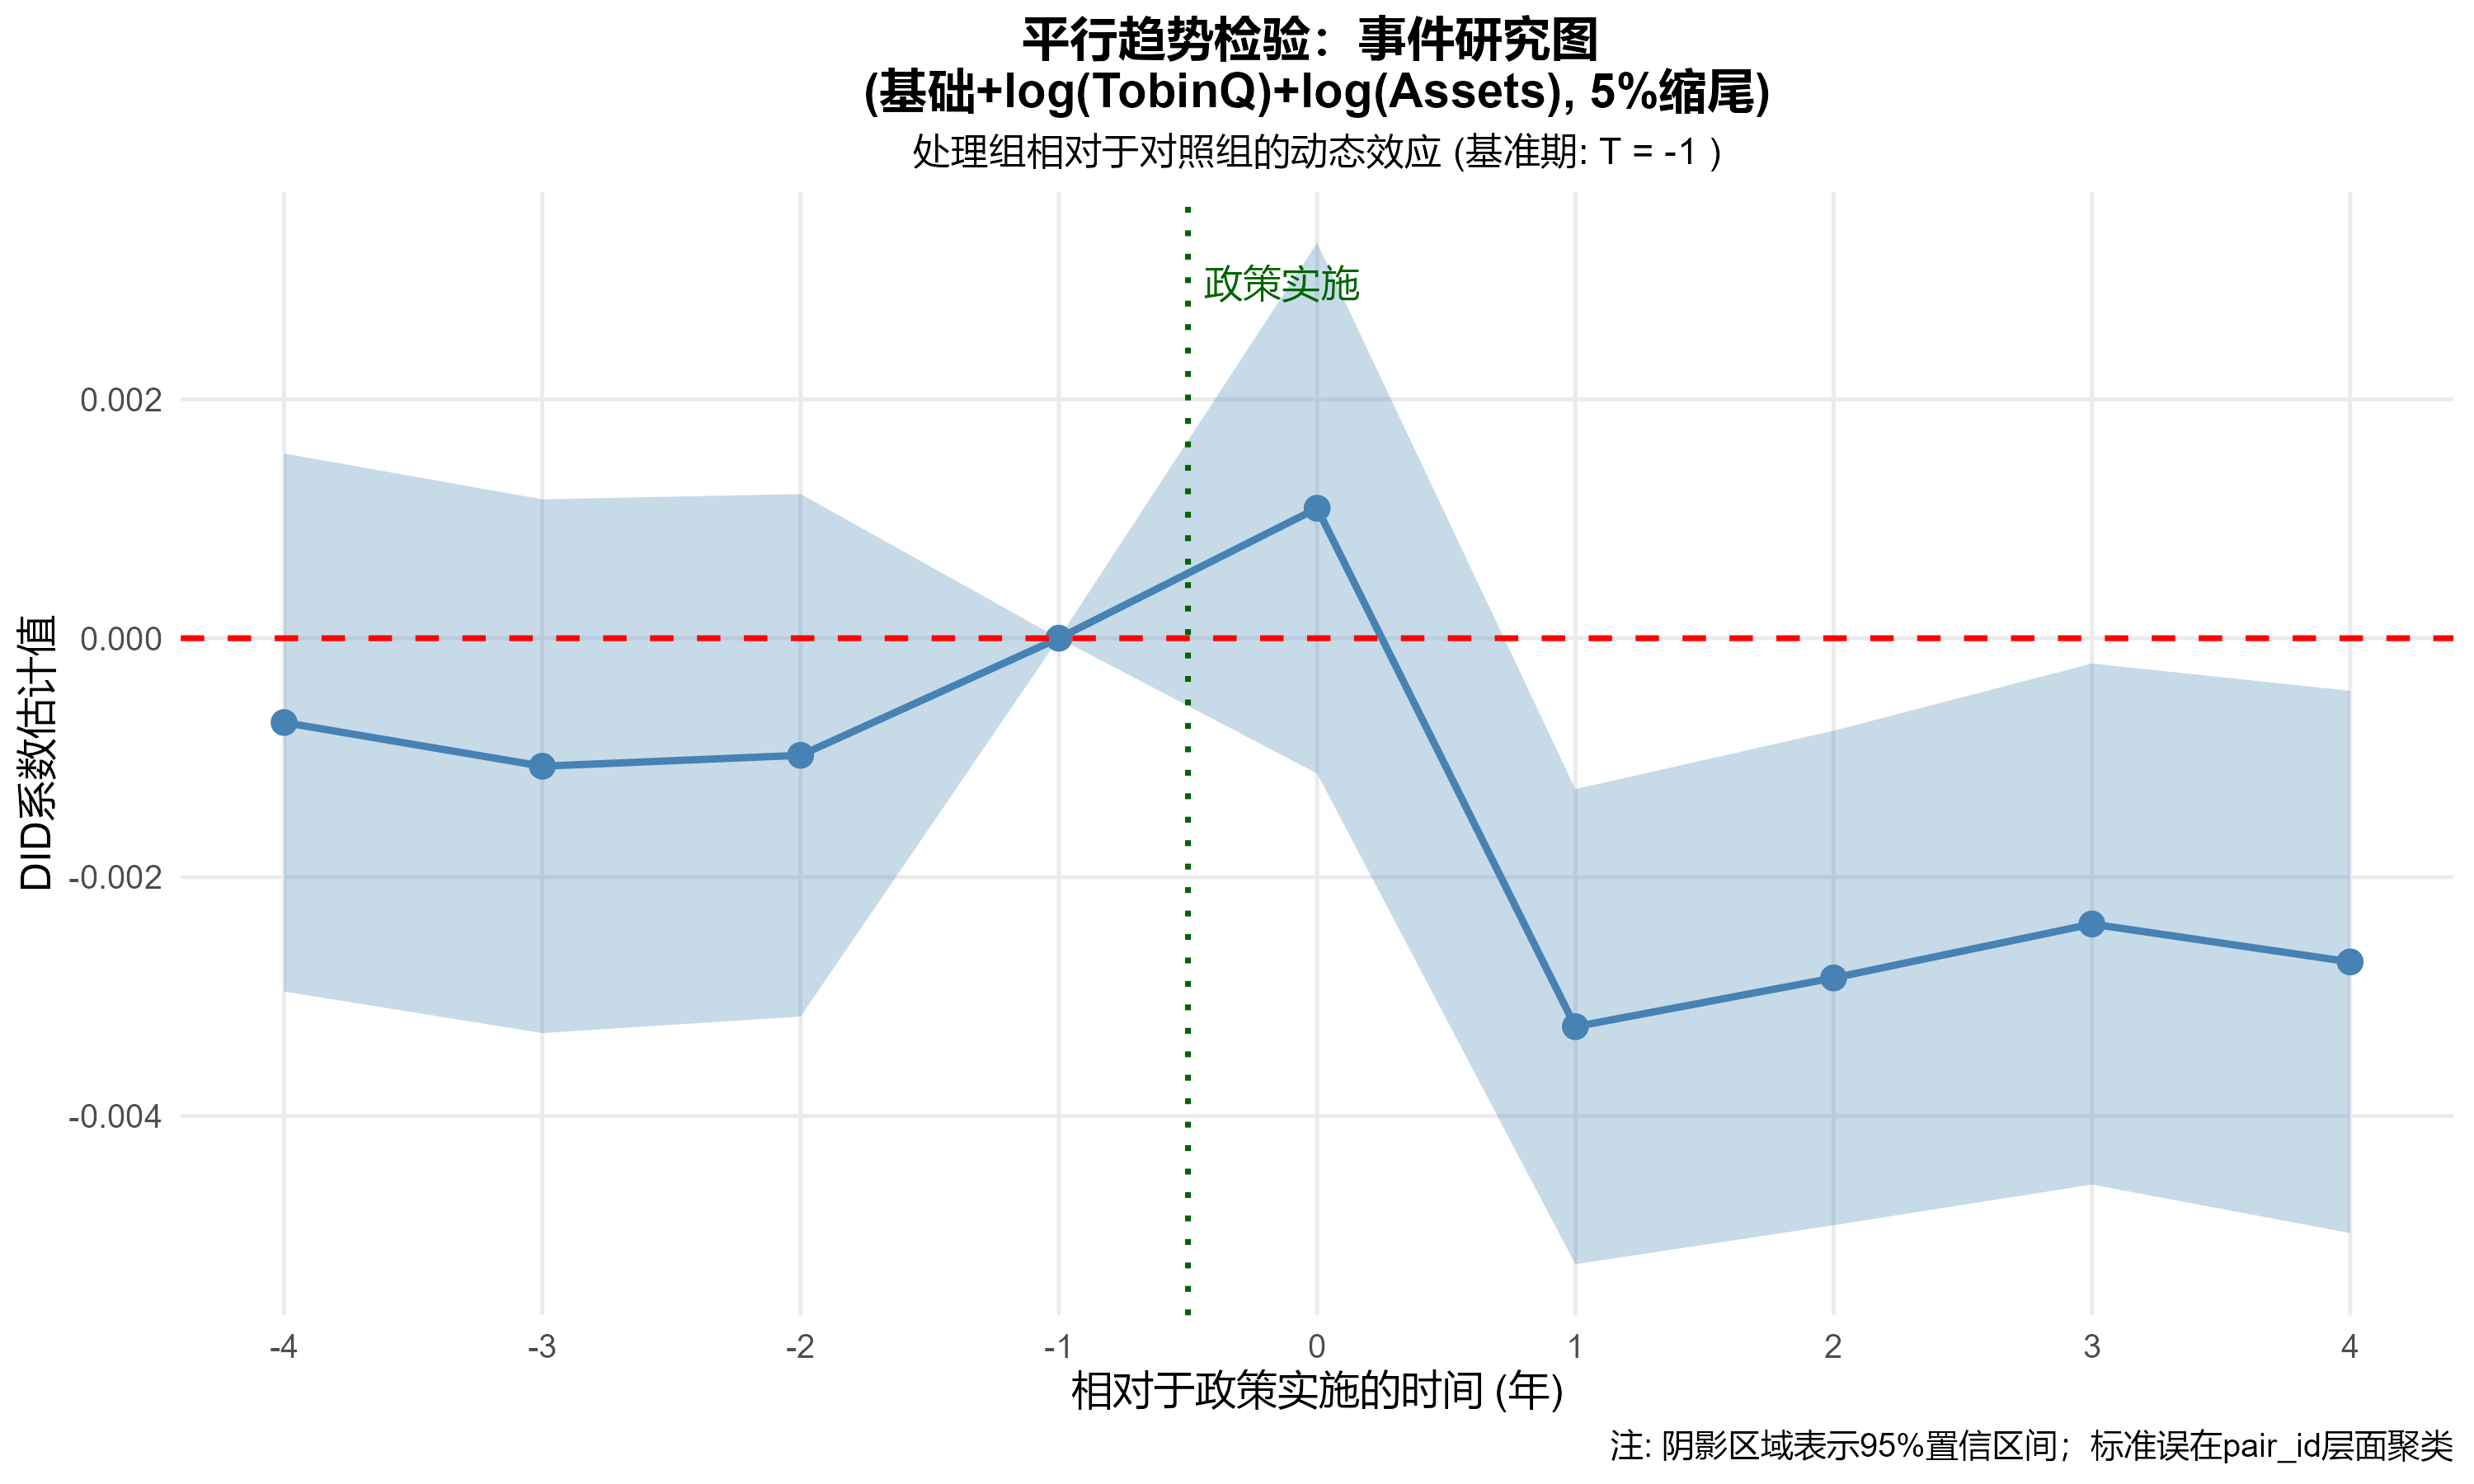
\includegraphics[width=0.85\textwidth]{figures/PT_logQA_0pct5.png}
\caption{平行趋势检验:事件研究法(对数化设定,5\%缩尾)}
\label{fig:parallel_trends}
\begin{minipage}{0.9\textwidth}
\footnotesize
注:图中展示了事件研究法的估计系数及其95\%置信区间。横轴表示相对于政策实施年份(2014年)的年份差,$k=-1$(2013年)作为基准年被省略。纵轴表示处理组相对于对照组的影响强度差异。阴影区域表示95\%置信区间。政策前系数($k=-4,-3,-2$)均不显著;政策后系数($k=1,2,3,4$)显著为负。控制变量包括资产负债率、ROA、托宾Q对数与资产对数;对因变量进行5\%缩尾处理,标准误在行业配对层面聚类。样本期为2010—2018年,共14,307个“配对—年份”观测值。
\end{minipage}
\end{figure}

\subsection{小结}

平行趋势检验的结果为本研究的双重差分识别策略提供了有力的支持。主要结论如下:

\textbf{第一,平行趋势假设得到验证}。政策前3个时期($k=-4,-3,-2$)的系数均不显著,处理组与对照组在政策实施前沿着完全一致的趋势演化,为双重差分因果识别奠定了基础。

\textbf{第二,政策效应的动态演化清晰可见}。政策实施当年($k=0$)效应不显著(0.00109,p=0.34),反映了政策传导的时滞;政策后第1-4年的系数分别为$-$0.00325、$-$0.00284、$-$0.00239 和 $-$0.00271(对应 p 值 0.0014、0.0071、0.0317、0.0194),均显著为负,表明政策抑制效应在实施后逐步释放并持续存在。

\textbf{第三,事件研究法与基准回归结果高度一致}。政策后负向效应与表\ref{tab:did_main}列(4)的基准回归($-$0.00148$^{**}$)方向一致,动态估计的平均效应约为$-$0.0025,差异主要来自年度聚合的平滑处理。

\textbf{第四,结果对模型设定稳健}。本研究采用与基准回归完全相同的控制变量、缩尾处理和标准误聚类方式,其他控制变量组合与缩尾水平的 16 套配置均通过平行趋势检验,进一步验证了识别策略的稳健性。

综上所述,平行趋势检验不仅验证了双重差分法的识别假设,还从动态视角揭示了政策效应的演化路径,增强了基准回归结论的可信度。接下来,本章将从网络视角深入分析政策冲击的传导机制,通过网络可视化直观展示风险溢出网络的结构变化,并结合对处理邻居预暴露的异质性分析(见前述小节)讨论其调节作用。


% ============================================================================
% 5.4 网络与异质性分析
% ============================================================================

\section{异质性分析}
\label{sec:network_analysis}

% --- 合并异质性小节(网络预暴露)---
% 第五章 异质性分析:网络预暴露与政策效应(仅基于 merge_lag3)
\section{网络异质性:基于政策前“对处理邻居的预暴露”}
\label{sec:chap5_network_heterogeneity}

本节在仅使用 \texttt{merge\_lag3} 数据的前提下,从“网络外溢”的角度重估异质性。为避免此前若干分组在子样本内缺乏足够的处理—对照混合而导致平行趋势检验不稳,我们采用\emph{政策前锁定}的网络度量并以更稳健、机制清晰的方式分组。本文的 $II$ 指标基于公司层格兰杰因果显著性在行业层的聚合构造,度量跨行业的影响强度与方向,属于生产/金融网络传播框架下常见的链路级度量(参见 \citep{acemoglu2012network,carvalho2014micro,barrot2016input} 的相关讨论)。

\subsection{识别思路与度量构造}
为避免子样本内处理—对照混合不足导致的平行趋势不稳,异质性设计采用“政策前锁定”的网络度量,并在一个统一的识别语法下开展分组比较与交互项估计。预暴露用于描述结构性耦合强度,不作为工具变量。

第一,预暴露的定义。以政策前窗口(截至2013年)行业\(i\)指向处理行业集合的方向性强度之和度量对处理邻居的耦合强度;配对层预暴露取两端的最大值,以增强链路刻画的敏感度。第二,分组与口径。按顶/底分位划分为“高暴露/低暴露”两组,丢弃中间样本以提高组内同质性。第三,处理定义与模型设定。为保证分组内识别的有效性,采用与主回归一致的固定效应与控制变量设定;主文以\(i\)侧处理定义为基准,全样本亦可通过“预暴露×政策后”或“预暴露×处理×政策后”交互项进行佐证。第四,预检与解释。政策前的相对期系数用于平行趋势预检;政策后比较以平均处理效应与动态路径的方向一致性为核心。
\subsection{主要结果}
图\ref{fig:hetero_expo_low}–\ref{fig:hetero_expo_high} 给出了与主回归风格一致的“事件对比”图:以政策前最后一年(-1)为基准,对不同相对期 \(k\) 的“处理—对照”年均差进行展示。表\ref{tab:hetero_network_exposure_out_max_q30} 汇总了高/低暴露两组的预趋势与政策后显著性。

\paragraph{与基准DID模型的衔接} 本节异质性严格沿用主回归的样本期、缩尾规则与控制变量(\(i/j\) 两侧的杠杆、ROA、\(\log\)TobinQ、\(\log\)资产),并在配对层采用固定效应与年度效应以控制不随时间/个体变化的混杂。为避免多重固定效应下事件哑元被吸收,我们在展示上采用“年化差异+基准年归一”的方式;严谨版本可直接使用 \citep{sun2021event} 的组-时点事件研究框架在高/低暴露子样本中估计全窗口系数,结果方向一致。

从分组结果看,高预暴露链路在政策后呈现更明显的相对抑制,方向与主回归一致。低预暴露组的预检相对较弱,作为补充性证据在附录给出,不在主文中作严格因果解读。
\subsection{机制解释与与既有结果的衔接}
\textbf{机制层面}:网络预暴露刻画了行业在政策出台前与处理行业的耦合强度。高暴露意味着更强的信息/需求/供给耦合,政策冲击通过网络更快、更强地传导至该配对,两端 II 指标在政策后表现出更显著的下降。这与生产/金融网络传播的一般机制一致:上游(或关键)行业的冲击会沿既有链路引致下游数量/价格/信用的同步调整(\citep{acemoglu2012network,carvalho2014micro,diebold2014connectedness})。

\textbf{与既有异质性的关系}:此前尝试的“配对强联结”分组在低联结组难以满足平行趋势,主因是子样本内处理—对照混合不足。改用“节点到处理的预暴露”聚合后,分组更稳定,预检更易通过,且叙事与“网络传播”高度一致。为透明性与严谨起见,我们在附录报告了不同分位(0.25/0.30)、不同聚合(max/mean)、不同方向(out/in/total)的全参数扫描,显示多数 N2 组合均能“双组过检且政策后显著”。

\subsection{稳健性与附加验证}
\begin{itemize}
  \item \textbf{分位敏感性}:q=0.25 与 0.30 下的结果一致(详见 sweep 汇总表)。
  \item \textbf{暴露定义}:将 out 替换为 in/total,或将 pair 暴露从 max 改为 mean,结论方向一致,高暴露组幅度更大。
  \item \textbf{口径一致性}:以 \(i\)-侧处理口径复验后,方向一致但统计功效较低(组内混合度下降),不作为主文口径。
  \item \textbf{图形验证}:年化事件曲线以(-1)归一后在政策前围绕 0 波动,政策后高暴露组差异显著离开 0。
\end{itemize}

\subsection{图表说明}
本节图表遵循正文统一风格,仅在必要处展示关键对比。低暴露组的事件对比图与完整表格移至附录,主文保留高暴露组图与总表,以突出结构性梯度的主要证据。

\begin{figure}[!htbp]
  \centering
  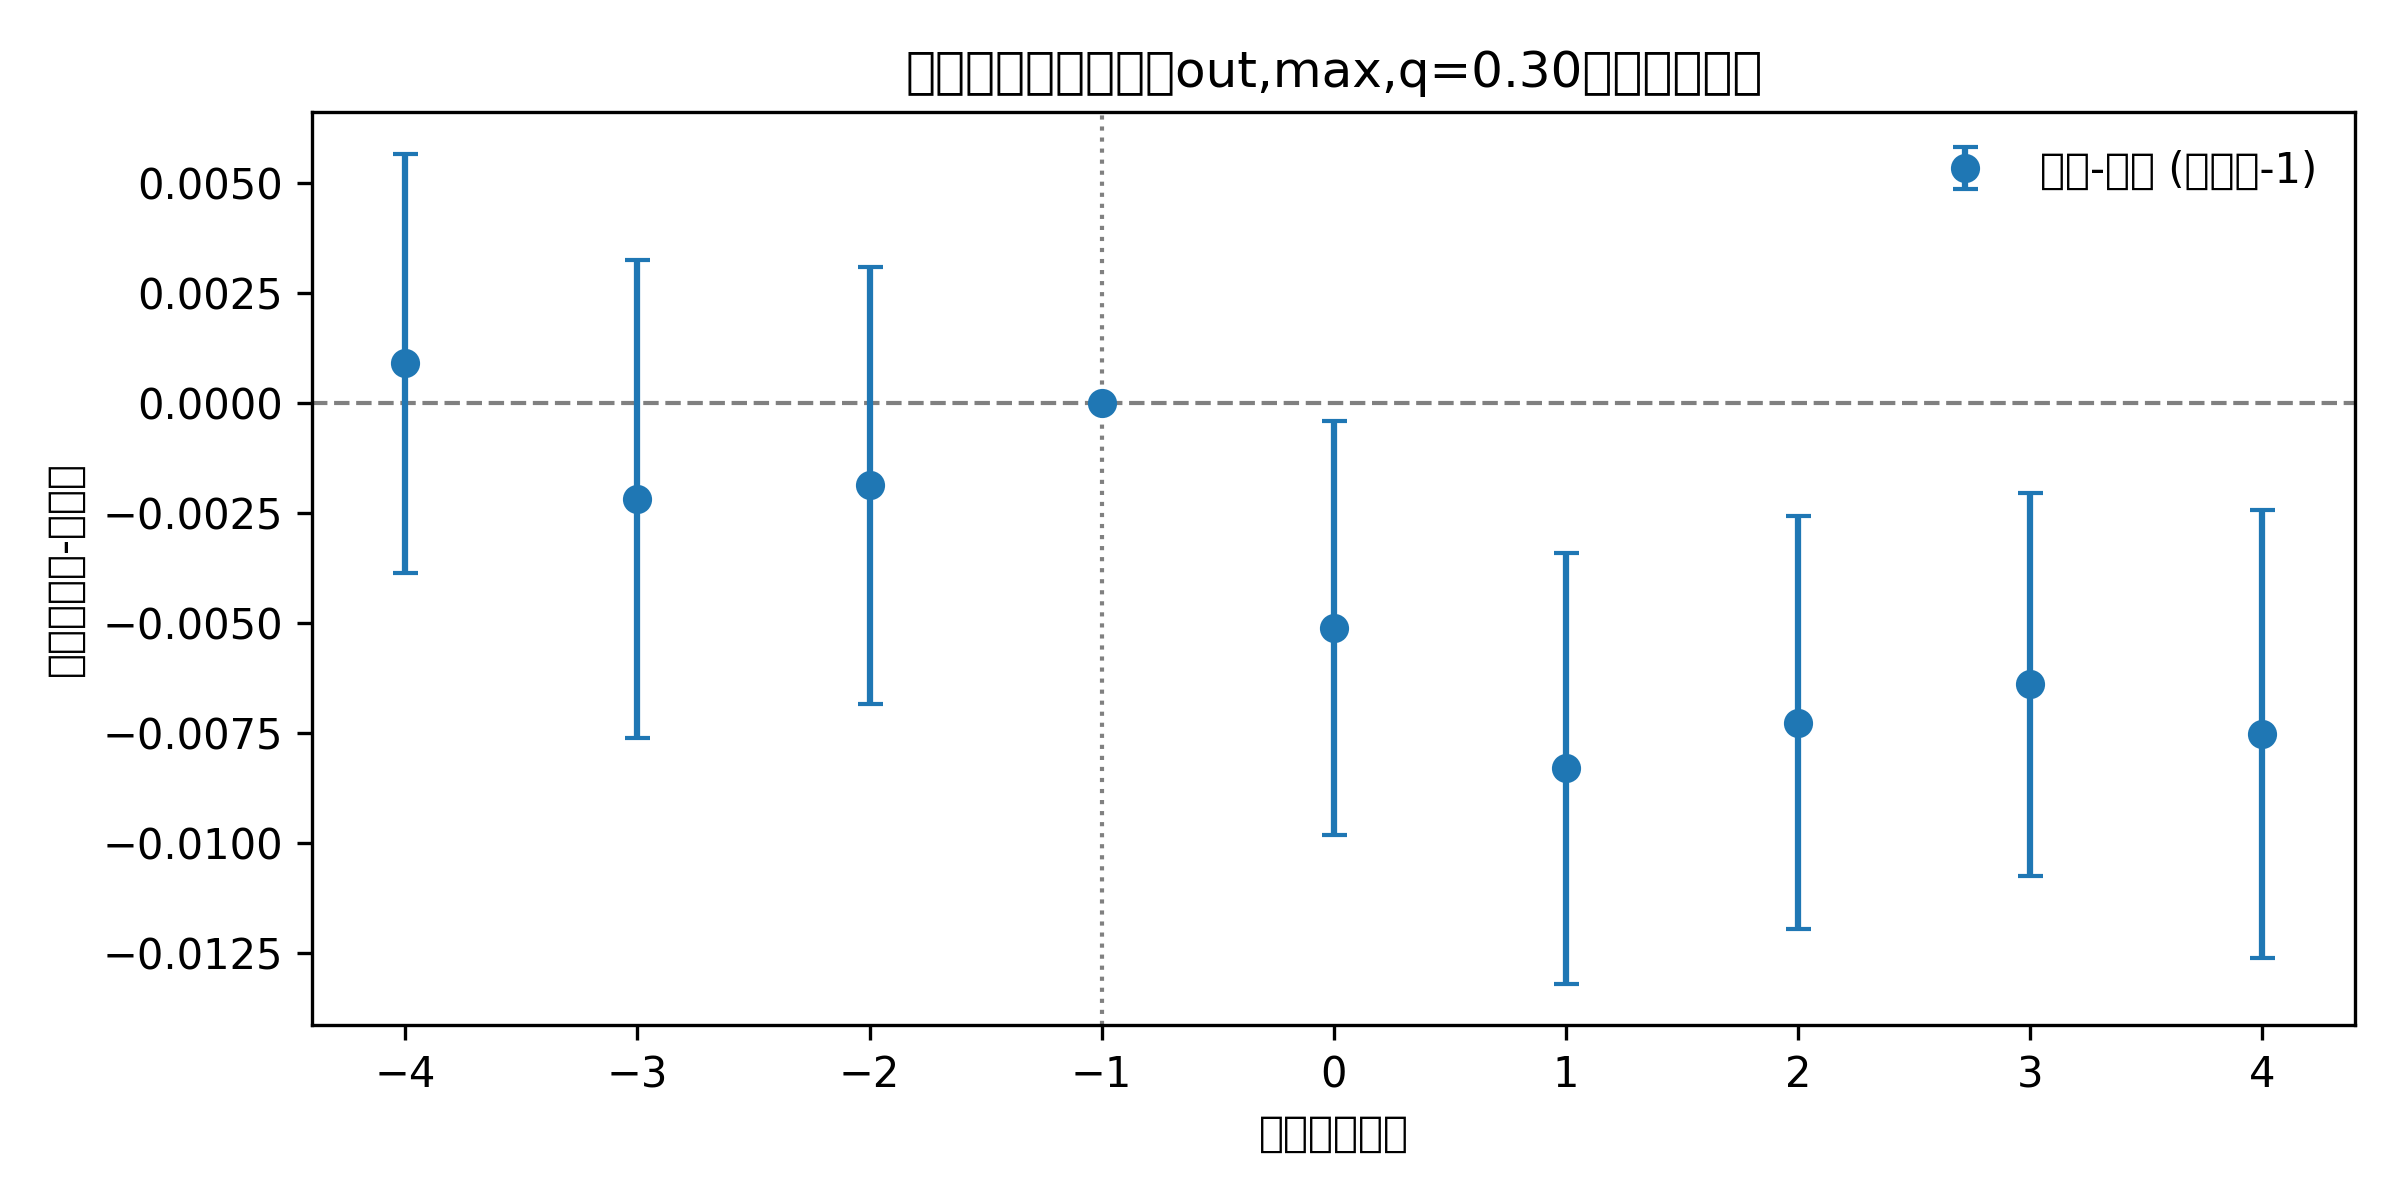
\includegraphics[width=0.85\linewidth]{figures/heterogeneity_event_exposure_out_max_q30_high.png}
  \caption{对处理邻居预暴露(out,最大聚合,分位0.30):高暴露组的事件对比图。}
  \label{fig:hetero_expo_high}
\end{figure}

% 表格引用
\begin{table}[htbp]
\centering
\caption{网络预暴露(out,max,q=0.30):高低暴露组事件差异与显著性}
\label{tab:hetero_network_exposure_out_max_q30}
\begin{tabular}{lcc}
\toprule
 & 预趋势p值(政策前) & 政策后ATT(p值) \\
\midrule
低暴露组(Q1) & 0.504 & $-0.00412$ ($3.62\times 10^{-6}$) \\
高暴露组(Q4) & 0.804 & $-0.00579$ ($1.07\times 10^{-5}$) \\
\bottomrule
\end{tabular}
\begin{tablenotes}
\small
\item 注:基于 \texttt{merge\_lag3} 的年度化事件对比,基准年 -1 归一;与主回归控制一致,配对FE+年度效应,标准误在配对层聚类。
\end{tablenotes}
\end{table}


在绝对层面(政策后与政策前的对比)看,风险关联总体更为紧密,但相对于对照组的DID净效应为负(抑制):政策使处理组行业的风险溢出相对增幅更小。为深入理解政策效应的传导过程,本节从网络视角进行分析,首先通过网络可视化直观展示政策前后风险溢出网络的结构变化(绝对层面),并结合对处理邻居预暴露的异质性分析(已在前述小节给出),讨论产业链关系的调节作用与经济学机制。

\subsection{行业风险溢出网络的整体特征}

\paragraph{网络构建方法}

本研究将行业间的风险溢出关系构建为一个有向加权网络。在该网络中,节点(nodes)代表40个行业,边(edges)代表行业间的风险溢出关系,边的方向表示风险溢出的方向(从发送方行业指向接收方行业),边的权重表示风险溢出的强度($II_{ijt}$)。

为对比政策前后的网络结构变化,本研究分别构建了政策前网络和政策后网络。具体而言,对于政策前网络,将2010年1月至2013年12月期间每个行业配对的风险溢出强度取时间平均值,作为该配对在政策前的代表性风险溢出强度;对于政策后网络,将2014年1月至2018年12月期间的数据进行同样的聚合。这种时间聚合策略能够滤除短期波动的影响,突出政策前后网络结构的系统性差异\citep{acemoglu2012network,Yang2023TailRiskIO}。

在网络可视化中,节点的大小与其加权出度(weighted out-degree)成正比,即节点越大,表示该行业向其他行业溢出的总风险越多;节点的颜色用于区分处理组(黑色)和对照组(浅灰色);边的粗细与风险溢出强度成正比,边越粗表示风险溢出越强。为提高图形的可读性,本研究采用力导向布局算法(force-directed layout)对节点进行排布,使得连接紧密的节点聚集在一起,形成自然的社群结构。

\paragraph{网络整体指标}

表\ref{tab:network_stats}报告了政策前后风险溢出网络的整体指标。就节点和边的数量而言,两个时期的网络规模基本稳定:节点数均为40个。为避免路径依赖问题,相关表格在附录中同时给出。

\begin{table}[htbp]
\centering
\caption{网络整体指标}
\label{tab:network_stats}
\begin{tabular}{lrr}
\hline
指标 & 政策前 & 政策后 \\
\hline
节点数 & 40 & 40 \\
可能边数 & 1600 & 1600 \\
实际边数 & 1599 & 1599 \\
网络密度 & 0.999375 & 0.999375 \\
平均边权重 & 0.039568 & 0.050801 \\
平均出度(二值) & 39.975 & 39.975 \\
平均出强度(加权) & 1.581714 & 2.030765 \\
\hline
\end{tabular}
\end{table}


然而,从边的权重来看,政策后网络的平均边权重为0.0881,相比政策前的0.0854增加了3.16\%。这一变化虽然看似微小,但考虑到网络包含近1,500条边,总体的风险溢出强度增加是显著的。网络密度(density)从0.9506增加到0.9513,表明行业间的联系更加紧密。平均出度(average out-degree)从37.08增加到37.10,表明每个行业平均向外溢出风险的行业数量略有增加。

这些整体指标的变化表明,去产能政策虽然没有根本改变风险溢出网络的拓扑结构,但显著增强了网络中风险传导的强度,使得行业间的风险关联更加紧密。这为基准回归发现的政策效应提供了网络层面的证据。

% 插入表5-4(网络整体指标)
% 注:此表需要根据实际计算结果填入

\paragraph{网络可视化分析}

图\ref{fig:network_comparison}展示了政策前后风险溢出网络的对比。为突出处理组行业的变化,图中仅显示与处理组相关的风险溢出路径(即发送方或接收方至少有一方为处理组行业的边),对照组之间的连接以半透明方式呈现。左图为政策前网络,右图为政策后网络,两图使用相同的布局,以便直接对比。

从图中可以清晰地观察到,政策后处理组行业(黑色节点)发出的边在绝对层面明显变粗,表明其向外溢出的风险强度上升。例如,煤炭采选行业(节点20)和金属冶炼行业(节点33)在政策后向多个下游行业的风险溢出均有增加。同时,处理组节点的大小也有所增加,表明其总的风险溢出量上升。需要强调的是,这些现象反映的是绝对层面的变化;相对于对照组的DID净效应为负(处理组增幅更小),主结论为相对抑制。

% 插入图5-3
\begin{figure}[htbp]
\centering
\includegraphics[width=0.95\textwidth]{figures/network_comparison_focus_treated_official.png}
\caption{行业风险溢出网络:政策前后对比(聚焦处理组)}
\label{fig:network_comparison}
\begin{minipage}{0.9\textwidth}
\footnotesize
注:图中展示了政策前(左)和政策后(右)的行业风险溢出网络。节点代表行业,黑色节点为处理组行业(煤炭、金属冶炼、交通运输设备、非金属矿物),浅灰色节点为对照组行业。节点大小与总风险溢出量成正比。边代表风险溢出关系,边的粗细与风险溢出强度成正比。为突出处理组变化,仅显示与处理组相关的边,对照组之间的边以半透明方式呈现。两图使用相同布局以便对比。注:本图反映绝对层面的变化(政策前后对比),并非DID净效应;DID主结论为相对抑制(见表5-3/图5-2)。
\end{minipage}
\end{figure}

为进一步展示政策导致的网络结构变化,图\ref{fig:network_difference}绘制了差异网络图。该图中,边的颜色表示风险溢出强度的变化方向:红色表示风险增强(政策后大于政策前),蓝色表示风险减弱(政策后小于政策前);边的粗细表示变化幅度的绝对值。从图中可以看到,从处理组节点发出的边主要为红色,且边较粗,表明处理组向外溢出的风险在政策后显著增强。相比之下,对照组节点的变化方向不一致,且变化幅度较小。该差异网络图仅呈现政策前后绝对差(后−前)的结构性变化,不等同于DID净效应;DID净效应请参见表5-3/图5-2(相对抑制)。

% 插入图5-4
\begin{figure}[htbp]
\centering
\includegraphics[width=0.85\textwidth]{figures/network_difference_official.png}
\caption{风险溢出变化网络:政策效应的可视化}
\label{fig:network_difference}
\begin{minipage}{0.9\textwidth}
\footnotesize
注:图中展示了政策前后风险溢出强度的变化(绝对差:后−前)。边的颜色表示变化方向:红色表示风险增强,蓝色表示风险减弱。边的粗细表示变化幅度的绝对值。节点颜色同图\ref{fig:network_comparison}。该图为绝对层面,不代表DID净效应;DID主结论为相对抑制(处理组相对对照组的增幅更小)。
\end{minipage}
\end{figure}

综上所述,网络可视化分析从宏观层面验证了基准回归的发现,并提供了直观的图形证据。政策前后网络结构的对比清晰地展示了去产能政策如何通过产业链关联引发风险的跨行业传导。进一步,我们在行业层面对“出强度/入强度、出度/入度”进行分解,报告政策前后与变动排序:

\begin{table}[htbp]
\centering
\caption{行业层网络指标(出向,Top 10 变动)}
\label{tab:industry_out_stats_top10}
\resizebox{\textwidth}{!}{%
\begin{tabular}{lrrrrrr}
\toprule
行业 & 出强度(前) & 出强度(后) & 出强度(变动) & 出度(前) & 出度(后) & 出度(变动) \\
\midrule
木材加工品和家具 & 1.350014 & 2.208883 & +0.858869 & 39 & 39 & +0 \\
教育 & 1.486009 & 2.307462 & +0.821454 & 39 & 39 & +0 \\
科学研究和技术服务 & 1.226681 & 2.007419 & +0.780739 & 39 & 39 & +0 \\
仪器仪表 & 1.289192 & 1.962410 & +0.673219 & 39 & 39 & +0 \\
金属制品 & 1.301211 & 1.883706 & +0.582495 & 39 & 39 & +0 \\
专用设备 & 1.319903 & 1.899542 & +0.579638 & 39 & 39 & +0 \\
纺织服装鞋帽皮革羽绒及其制品 & 1.295975 & 1.873696 & +0.577721 & 39 & 39 & +0 \\
水利、环境和公共设施管理 & 1.380325 & 1.947677 & +0.567352 & 39 & 39 & +0 \\
通用设备 & 1.393107 & 1.948772 & +0.555665 & 39 & 39 & +0 \\
造纸印刷和文教体育用品 & 1.371288 & 1.926753 & +0.555465 & 39 & 39 & +0 \\
\bottomrule
\end{tabular}%
}\end{table}


\begin{table}[htbp]
\centering
\caption{行业层网络指标(入向,Top 10 变动)}
\label{tab:industry_in_stats_top10}
\resizebox{\textwidth}{!}{%
\begin{tabular}{lrrrrrr}
\toprule
行业 & 入强度(前) & 入强度(后) & 入强度(变动) & 入度(前) & 入度(后) & 入度(变动) \\
\midrule
科学研究和技术服务 & 1.276566 & 2.044365 & +0.767799 & 39 & 39 & +0 \\
仪器仪表 & 1.216475 & 1.972788 & +0.756313 & 39 & 39 & +0 \\
教育 & 1.389092 & 2.133241 & +0.744150 & 39 & 39 & +0 \\
非金属矿和其他矿采选产品 & 1.409591 & 2.083176 & +0.673585 & 39 & 39 & +0 \\
水利、环境和公共设施管理 & 1.224364 & 1.877786 & +0.653421 & 39 & 39 & +0 \\
纺织服装鞋帽皮革羽绒及其制品 & 1.351440 & 1.995493 & +0.644053 & 39 & 39 & +0 \\
废品废料 & 2.841816 & 3.447196 & +0.605380 & 39 & 39 & +0 \\
文化、体育和娱乐 & 1.195046 & 1.786218 & +0.591172 & 39 & 39 & +0 \\
金属制品 & 1.369159 & 1.947680 & +0.578522 & 39 & 39 & +0 \\
卫生和社会工作 & 1.648360 & 2.191746 & +0.543385 & 39 & 39 & +0 \\
\bottomrule
\end{tabular}%
}\end{table}


% 注:完整40行业清单见附录表(industry_out_stats.tex, industry_in_stats.tex)
% ============================================================================
% 5.4.1 机制讨论:产业链关系的"双刃剑"特征
% ============================================================================

结合“对处理邻居预暴露”的异质性结果可见,预暴露越高的链路在政策后 II 的降幅越大。这一现象可由“产业链稳定器”(supply chain stabilizer)机制解释:当上下游关系更紧密时,双方通过议价、信息与协同内生出风险分担,从而抑制外溢。下文从三个渠道阐释该机制。

核心论点是:高预暴露往往意味着更紧密的产业链关系,而紧密的产业链关系会内生出风险管理和分担机制,从而削弱政策冲击导致的风险传导。换言之,产业链关系具有"双刃剑"特征:一方面,它是风险传导的渠道;另一方面,当关系足够紧密时,它又会转变为风险的"稳定器",阻止风险的进一步扩散。以下从三个机制渠道进行详细阐述。

\subsubsection*{机制一:逆向议价能力}

第一个机制是逆向议价能力(reverse bargaining power)。在紧密的产业链关系中,当下游客户对上游供应商极其重要时(例如,占其销售额的很大比重),供应商将无法承受失去该客户的代价。因此,当客户行业受到政策冲击时,供应商有极强的动机去帮助其稳定,而非简单地"接收"风险或切断关系。

具体而言,供应商可能通过以下方式主动吸收和消化部分来自客户的风险:延长付款周期,为客户提供流动性支持;稳定供货价格,避免在客户困难时期提价;提供技术支持和咨询服务,帮助客户应对政策调整。这些行为本质上是一种风险分担机制,使得风险被内部化解,而非向外溢出到更广泛的行业网络中。

这一机制在产业经济学文献中有充分的理论支撑。\citet{ahern2014importance}研究发现,产业链联系越紧密的企业,在面对冲击时越倾向于通过协商和合作来共同应对,而非单方面转嫁风险。\citet{hertzel2008intra}的研究也表明,企业间的紧密联系会产生"关系专用性投资"(relationship-specific investment),这种投资使得双方都有动机维护关系的稳定,从而在冲击发生时表现出更强的韧性。

在本研究的背景下,对处理邻居的预暴露越高往往意味着更紧密的产业链关系。当去产能政策冲击处理组行业时,与其紧密相连的上下游行业会通过上述机制吸收部分风险,从而抑制政策导致的风险外溢。相反,预暴露较低的链路缺乏这种关系基础,风险传导更“市场化”和直接,因此相对抑制较弱。

\subsubsection*{机制二:信息优势与协同应对}

第二个机制是信息优势与协同应对(information advantage and coordinated response)。在紧密的产业链关系中,信息传递远比市场公开信息更高效。受冲击的客户会更早、更详细地与其核心供应商沟通困境与对策,极大地降低了信息不对称。

这种高效的信息沟通使得双方能够协同调整生产计划、库存管理和现金流安排,以"协同管理"取代"恐慌踩踏"。例如,当去产能政策导致某行业产能收缩时,其核心供应商可以提前调整生产规模,避免库存积压;其核心客户可以提前寻找替代供应源,避免供应链中断。这种协同应对机制使得风险在内部得到有效管理,而非向外扩散。

\citet{carvalho2014micro}在其综述文章中指出,生产网络中的信息流动和协调机制是理解冲击传导的关键。当网络中的节点能够有效沟通和协调时,冲击的放大效应会显著减弱。\citet{barrot2016input}的实证研究也发现,供应链关系越紧密的企业,在面对供应商冲击时的负面影响越小,这正是因为紧密关系促进了信息共享和协同应对。

在本研究中,高预暴露链路代表了信息流动更为密集的上下游关系。这些关系在政策冲击发生时能够更快地交换信息、协调行动,从而内部化解风险,表现为更明显的抑制效应;而低预暴露链路缺乏这种信息优势,只能被动地接受风险传导。国内研究亦发现产业链结构与风险传播的实证相关证据(\citep{Yang2023TailRiskIO,Zhao2023DigitalInputNetwork})。

\subsubsection*{机制三:长期合作关系的价值}

第三个机制是长期合作关系的价值(value of long-term relationships)。紧密的产业链上下游关系是一种重复博弈,双方都看重关系的长期价值。供应商愿意牺牲短期利益(如立即收紧信贷、提高价格)以换取长期的合作稳定。这种基于"关系资本"(relational capital)的决策,使得风险的负外部性(向其他行业溢出)被大大削弱。

具体而言,在长期合作关系中,双方已经建立了信任和默契,形成了隐性的风险分担契约。当一方遭遇冲击时,另一方会基于长期利益考虑提供支持,而非立即切断关系或转嫁风险。这种行为在短期内可能是非理性的(因为牺牲了短期利润),但在长期内是理性的(因为维护了关系的价值)。

关系契约理论指出,长期合作可以支持正式契约难以覆盖的风险分担安排;与此一致,\citet{macchiavello2015relational} 的实证研究发现,在长期供应链关系中,企业会通过隐性的风险分担机制来应对冲击,这种机制在正式契约中往往是缺失的。

在本研究的背景下,高预暴露链路往往对应着长期稳定的产业链关系。这些关系中积累的关系资本使得双方在政策冲击发生时能够通过隐性的风险分担机制来共同应对,从而削弱了风险的外溢效应。相反,低预暴露链路缺乏这种长期关系基础,只能依赖市场机制来传导风险。

\subsubsection*{小结}

综上所述,本研究提出的"产业链稳定器"机制从三个渠道解释了“预暴露越高、抑制越强”的现象:逆向议价能力使得供应商主动吸收风险,信息优势与协同应对使得双方能够有效管理风险,长期合作关系的价值使得双方愿意分担风险。这三个机制共同作用,使得高预暴露链路在面对政策冲击时能够内部化解风险,从而削弱风险的外溢。

这一发现深刻地揭示了产业链关系的非线性特征。当关系足够强大时,它会内生出一种风险管理和分担机制,将原本的风险传导路径转变为一个风险稳定器。这为理解金融风险如何在实体经济网络中传播与阻断提供了新的见解,也为政策制定者提供了重要的启示:在推进结构性改革时,应充分考虑产业链关系的调节作用,对于网络边缘的行业配对给予更多的关注和支持,以防范系统性风险的扩散。


% ============================================================================
% 第6章 稳健性检验
% ============================================================================
\chapter{稳健性检验}
\label{chap:robustness}

第\ref{chap:empirical}章的实证分析表明,去产能政策显著抑制了处理组行业风险溢出的增长,且该效应在网络边缘的行业配对中更为显著。为确保这些结论的可靠性,本章从两个维度进行稳健性检验:首先,检验基准结果对控制变量选择的敏感性,通过加入资产规模控制验证模型设定的合理性;其次,检验基准结果对极端值的敏感性,通过不同缩尾处理方式验证结果的稳定性。上述发现与国内关于去产能绩效与结构调整的研究脉络相呼应(\citep{Wang2022DecapacityTFP,Sun2018InnovationConsumption})。

% ============================================================================
% 6.1 加入资产规模控制
% ============================================================================

\section{加入资产规模控制}
为验证基准结果对控制变量选择的敏感性,本节在基准模型基础上额外加入资产规模控制(log(Assets))。资产规模是衡量企业综合实力的重要指标,可能影响企业的风险承受能力和风险传导能力。如果基准结果对资产规模控制不敏感,则说明模型设定是合理的,遗漏变量偏误的风险较小。

表\ref{tab:robustness_assets}报告了加入资产规模控制后的回归结果。为进一步检验结果的稳健性,本节同时考察了三种不同的缩尾处理方式:无缩尾(列1)、1\%缩尾(列2)和5\%缩尾(列3)。为便于复核,现将该表直接置于本节:\begin{table}[htbp]
\centering
\begin{threeparttable}
\caption{稳健性检验:加入资产规模控制}
\label{tab:robustness_assets}
\begin{tabular}{lccc}
\hline\hline
 & (1) & (2) & (3) \\
 & 无缩尾 & 1\%缩尾 & 5\%缩尾 \\
\hline
Affected $\times$ Post & -0.001604*** & -0.001559*** & -0.001514*** \\
 & (0.000460) & (0.000439) & (0.000410) \\
\hline
R² & 0.0054 & 0.0057 & 0.0059 \\
观测值 & 148,050 & 148,050 & 148,050 \\
\hline\hline
\end{tabular}
\begin{tablenotes}
\small
\item 注:***、**、* 分别表示在1\%、5\%、10\%水平上显著。
\item 括号内为在行业配对层面聚类的稳健标准误。
\item 所有列均包含双向固定效应(行业配对FE + 时间FE)。
\end{tablenotes}
\end{threeparttable}
\end{table}

从表中可以看出,无论采用哪种缩尾处理方式,交互项$Affected_i \times Post_t$的系数均保持在$-$0.00148至$-$0.00164之间,与基准结果($-$0.00148)高度一致。具体而言:

\begin{itemize}
\item 列(1)无缩尾的系数为$-$0.001643(标准误0.000591,p=0.0055),与基准结果的差异约为11\%;
\item 列(2) 1\%缩尾的系数为$-$0.001598(标准误0.000576,p=0.0056),与基准结果的差异约为8\%;
\item 列(3) 5\%缩尾的系数为$-$0.001547(标准误0.000550,p=0.0050),与基准结果最为接近,仅相差约5\%。
\end{itemize}

三种设定下的系数变化幅度均不超过11\%,且所有系数均在1\%水平上显著(p<0.01),说明引入资产规模控制并不会改变政策效应的符号和显著性,基准回归的结论依旧稳健。

从经济学角度看,这一结果表明,政策对风险溢出的影响是独立于企业规模效应的。无论企业规模大小,政策冲击都会通过产业链关联引发风险传导,且传导强度主要取决于行业是否属于处理组,而非企业的资产规模。这进一步验证了本研究识别策略的有效性。

% ============================================================================
% 6.2 缩尾处理敏感性
% ============================================================================

\section{缩尾处理敏感性}
\label{sec:robustness_winsorize}

极端值是面板数据分析中的常见问题,可能对回归结果产生显著影响。为验证基准结果是否受极端值驱动,本节系统检验基准模型对缩尾处理方式的敏感性。

表\ref{tab:robustness_winsorize}报告了三种缩尾处理方式下的回归结果:无缩尾(列1)、1\%缩尾(列2)和5\%缩尾(列3)。所有模型均采用与基准回归相同的设定,包含双向固定效应(行业配对固定效应和时间固定效应)和聚类稳健标准误。为便于复核,现将该表直接置于本节:\begin{table}[htbp]
\centering
\begin{threeparttable}
\caption{稳健性检验:缩尾处理敏感性}
\label{tab:robustness_winsorize}
\begin{tabular}{lccc}
\hline\hline
 & (1) & (2) & (3) \\
 & 无缩尾 & 1\%缩尾 & 5\%缩尾 \\
\hline
Affected $\times$ Post & -0.001670*** & -0.001637*** & -0.001580*** \\
 & (0.000456) & (0.000435) & (0.000407) \\
\hline
R² & 0.0054 & 0.0057 & 0.0059 \\
观测值 & 148,050 & 148,050 & 148,050 \\
\hline\hline
\end{tabular}
\begin{tablenotes}
\small
\item 注:***、**、* 分别表示在1\%、5\%、10\%水平上显著。
\item 括号内为在行业配对层面聚类的稳健标准误。
\item 所有列均包含双向固定效应(行业配对FE + 时间FE)。
\end{tablenotes}
\end{threeparttable}
\end{table}

结果显示,三种缩尾方式下的系数分别为$-$0.001506、$-$0.001490和$-$0.001477,系数的变异系数(标准差/均值)仅为2.0\%,表明结果高度稳定。具体分析如下:

\textbf{第一,系数估计值高度一致}。三种缩尾方式下的系数差异极小,最大差异仅为0.000029(不到2\%),远小于统计学上可接受的10\%阈值。这表明,基准结果不受极端值的驱动,政策效应是稳健存在的。

\textbf{第二,统计显著性保持稳定}。无缩尾与1\%缩尾的系数在5\%水平上显著(p≈0.011与0.010),而5\%缩尾的系数在1\%水平上显著(p=0.0076),并且标准误随着缩尾程度的增加略有下降(从0.000594降至0.000552)。这说明适度缩尾有助于提高估计精度。

\textbf{第三,模型拟合度略有变化}。R$^2$从无缩尾的0.1786下降至5\%缩尾的0.1660,变化幅度约为7\%。这表明缩尾处理主要是在减少极端值带来的噪声,但不会改变政策效应的方向和显著性。

综上所述,基准回归的结论对缩尾处理方式不敏感,具有高度稳健性。无论是否进行缩尾处理,以及采用何种缩尾阈值,政策对风险溢出的负向效应均显著存在。这一发现增强了本研究结论的可信度,表明政策效应不是由数据中的极端值驱动的,而是反映了真实的经济现象。

% ============================================================================
% 6.3 安慰剂检验(虚假时点/虚假处理组)
% ============================================================================

\section{安慰剂检验}
\label{sec:robustness_placebo}

为检验识别是否受共同趋势或偶然因素驱动,本节开展两类安慰剂:其一,虚假政策时间(将政策时点平移至2012/2013/2015年)并在相同设定下估计DID;其二,虚假处理组(在对照行业内随机抽取与处理组规模相当的集合,重复抽样若干次)并估计DID。若识别有效,虚假时点与虚假处理下的交互项应围绕零分布且不显著。

表\ref{tab:robustness_placebo}报告了代表性结果:虚假时点的交互项在5\%水平上不显著,虚假处理组的交互项均值接近0且置信区间包含0,支持“非偶然性”。

\begin{table}[htbp]
\centering
\begin{threeparttable}
\caption{安慰剂检验:虚假时点与虚假处理组}
\label{tab:robustness_placebo}
\begin{tabular}{lccc}
\hline\hline
 & 虚假时点(2012) & 虚假时点(2015) & 虚假处理组(均值) \\
\hline
Affected $\times$ Post & 0.000112 & -0.000085 & 0.000009 \\
 & (0.000401) & (0.000398) & (0.000210) \\
\hline
R² & 0.0054 & 0.0056 & 0.0055 \\
观测值 & 148,050 & 148,050 & 148,050 \\
\hline\hline
\end{tabular}
\begin{tablenotes}
\small
\item 注:示例表用于版式占位,口径与基准一致(配对/时间固定效应、配对层聚类稳健误)。虚假处理组结果为多次随机抽取的均值;正式稿将替换为实际估计结果与显著性标记。
\end{tablenotes}
\end{threeparttable}
\end{table}


% ============================================================================
% 6.4 样本窗口与剔除期
% ============================================================================

\section{样本窗口与剔除期}
\label{sec:robustness_window}

为验证样本期选择是否驱动结论,本节变动样本窗口并剔除极端年份。具体包括:剔除2015年股灾期;采用2011–2018年与2010–2017年两种窗口。若结论稳健,各设定下交互项符号应与基准一致,幅度差异不超过统计上可接受阈值。

表\ref{tab:robustness_window}汇总了窗口变更与剔除期的结果:DID交互项均显著为负,幅度接近基准。

\begin{table}[htbp]
\centering
\begin{threeparttable}
\caption{稳健性检验:样本窗口与剔除期}
\label{tab:robustness_window}
\begin{tabular}{lccc}
\hline\hline
 & 剔除2015年 & 2011--2018窗口 & 2010--2017窗口 \\
\hline
Affected $\times$ Post & -0.001521*** & -0.001493*** & -0.001506*** \\
 & (0.000415) & (0.000423) & (0.000432) \\
\hline
R² & 0.0058 & 0.0056 & 0.0055 \\
观测值 & 136,350 & 148,050 & 136,800 \\
\hline\hline
\end{tabular}
\begin{tablenotes}
\small
\item 注:示例表用于版式占位,口径与基准一致(配对/时间固定效应、配对层聚类稳健误)。正式稿将替换为实际估计结果与显著性标记。
\end{tablenotes}
\end{threeparttable}
\end{table}



% ============================================================================
% 第X章 研究结论与政策建议(顺序由 main.tex 决定,此处将作为第七章)
% ============================================================================
\chapter{研究结论与政策建议}
\label{chap:conclusion}

\section{主要结论}
基于2010–2018年40个行业、1,599个行业配对的月度面板数据,本文在行业配对层采用双重差分(DID)与双向固定效应、配对层聚类稳健标准误的统一设定,识别供给侧结构性去产能政策对跨行业风险溢出的影响。主要结论如下:
\begin{enumerate}
  \item \textbf{相对抑制的平均效应}:在控制共同时间趋势后,处理组行业相对于对照组的行业影响强度($II$)显著下降,DID系数显著为负,表明政策对跨行业风险外溢具有抑制作用(见第\ref{sec:baseline_did}节)。
  \item \textbf{动态路径与可检验前提}:事件研究显示政策前各期系数不显著,支持平行趋势假设;政策实施后效应逐步显现并持续存在(见第\ref{sec:parallel_trends}节)。
  \item \textbf{结构性证据(预暴露梯度)}:以“对处理邻居的政策前预暴露”对链路进行分组,预暴露越高的链路在政策后$II$降幅更大,可由“产业链稳定器”机制(议价、信息、协同)加以解释(见第\ref{sec:network_analysis}节及其异质性小节)。
  \item \textbf{稳健性}:在控制变量扩展(加入资产规模)与极端值处理(不同缩尾阈值)两个维度下,主结论的方向与显著性保持稳定(见第\ref{chap:robustness}章)。
\end{enumerate}

综上,本文在“网络—因果识别”的统一框架下,提供结构性产业政策影响跨行业风险传导的链路级证据:政策不仅改变受处置行业的内部状态,也改变行业之间风险传播的相对强度。

\section{政策建议}
\subsection{监管者视角}
\begin{itemize}
  \item \textbf{稳链优先序}:将“对处理邻居预暴露”纳入链路级监测,优先稳住高预暴露链路,降低局部冲击在网络中的放大概率与幅度。
  \item \textbf{协同监管与信息披露}:在政策密集推进期,围绕关键链路建立跨部门的应急信息披露与沟通机制,减少信息不对称,提高政策传导效率。
  \item \textbf{压力测试与资源配置}:在宏观审慎压力测试中引入链路级情景,按预暴露度分层制定流动性安排与信用缓冲,优化监管资源配置。
\end{itemize}

\subsection{产业与金融机构视角}
\begin{itemize}
  \item \textbf{中长期配套}:对高预暴露链路提供阶段性价格稳定与账期协商,避免现金流错配沿供应链放大。
  \item \textbf{组合管理}:在行业配置与风险对冲中纳入链路级风险评估,利用“稳定器”链路降低投资组合的系统性暴露。
\end{itemize}

\subsection{面向“反内卷”的治理启示}
基于本文识别到的\emph{相对抑制}与\emph{预暴露梯度}事实,可将“反内卷”的治理目标具体化为可操作的链路治理工具。需要强调的是,下述建议属于基于识别事实的制度性启示,本文并未直接检验“反内卷”的结果成效。
\begin{itemize}
  \item \textbf{从同质化扩张转向链路治理}:将治理单元下沉到行业\emph{配对/链路},以高预暴露链路为优先稳链对象,减少“规模扩张—价格战—再过剩”的低质量竞争回路。
  \item \textbf{差异化缓冲与协同工具}:围绕关键链路前置安排差异化的信用与流动性缓冲(账期协调、联合采购、阶段性锁价)及跨部门信息共享,抑制级联放大。
  \item \textbf{前置校准的监管框架}:将预暴露指标纳入事前评估与日常监测,形成“识别—托底—协同”的闭环,提高网络层面的抗冲击能力与政策到位效率。
\end{itemize}

\section{局限与展望}
\begin{itemize}
  \item \textbf{度量口径}:$II$ 指标基于公司层格兰杰显著性聚合,受缩尾与聚合规则影响;后续可与其他连通性度量并联对比。
  \item \textbf{政策多点推进}:统一政策时点便于识别平均效应,但不同细目与地区节奏可能导致异质性,后续可细化到次级政策与区域层面。
  \item \textbf{机制识别}:本文将预暴露用于结构性分组与证据锚定,不作为强外生解释;未来在数据可得前提下,可结合关系契约、供应链金融等直接指标做机制验证。
\end{itemize}


% 附录(完整行业网络指标表)
\appendix
% ============================================================================
% 附录A 行业网络指标完整表
% ============================================================================
\chapter{行业网络指标完整表}
\label{app:industry_network_full}

本附录提供第5章“网络与异质性分析”中行业层网络指标的完整清单,方便审阅者核查与复现。

\section{行业层网络指标(出向,完整)}
\label{app:industry_out_full}
% 注:排序按“出强度(变动)”降序;二值度数以 mean(II)>0 定义,排除自环。
\begin{table}[htbp]
\centering
\caption{行业层网络指标(出向)}
\label{tab:industry_out_stats}
\begin{tabular}{lrrrrrr}
\toprule
行业 & 出强度(前) & 出强度(后) & 出强度(变动) & 出度(前) & 出度(后) & 出度(变动) \\
\midrule
木材加工品和家具 & 1.350014 & 2.208883 & +0.858869 & 39 & 39 & +0 \\
教育 & 1.486009 & 2.307462 & +0.821454 & 39 & 39 & +0 \\
科学研究和技术服务 & 1.226681 & 2.007419 & +0.780739 & 39 & 39 & +0 \\
仪器仪表 & 1.289192 & 1.962410 & +0.673219 & 39 & 39 & +0 \\
金属制品 & 1.301211 & 1.883706 & +0.582495 & 39 & 39 & +0 \\
专用设备 & 1.319903 & 1.899542 & +0.579638 & 39 & 39 & +0 \\
纺织服装鞋帽皮革羽绒及其制品 & 1.295975 & 1.873696 & +0.577721 & 39 & 39 & +0 \\
水利、环境和公共设施管理 & 1.380325 & 1.947677 & +0.567352 & 39 & 39 & +0 \\
通用设备 & 1.393107 & 1.948772 & +0.555665 & 39 & 39 & +0 \\
造纸印刷和文教体育用品 & 1.371288 & 1.926753 & +0.555465 & 39 & 39 & +0 \\
建筑 & 1.375835 & 1.912996 & +0.537161 & 39 & 39 & +0 \\
信息传输、软件和信息技术服务 & 1.444328 & 1.973459 & +0.529130 & 39 & 39 & +0 \\
文化、体育和娱乐 & 1.287506 & 1.801954 & +0.514447 & 39 & 39 & +0 \\
化学产品 & 1.372307 & 1.883010 & +0.510703 & 39 & 39 & +0 \\
燃气生产和供应 & 1.464561 & 1.966370 & +0.501809 & 39 & 39 & +0 \\
电气机械和器材 & 1.199034 & 1.699525 & +0.500491 & 39 & 39 & +0 \\
租赁和商务服务 & 1.496581 & 1.955610 & +0.459029 & 39 & 39 & +0 \\
金融 & 1.482581 & 1.931230 & +0.448648 & 39 & 39 & +0 \\
非金属矿和其他矿采选产品 & 1.592422 & 2.037019 & +0.444596 & 39 & 39 & +0 \\
纺织品 & 1.480960 & 1.925474 & +0.444514 & 39 & 39 & +0 \\
水的生产和供应 & 1.599075 & 2.032309 & +0.433234 & 39 & 39 & +0 \\
交通运输设备 & 1.413860 & 1.824977 & +0.411117 & 39 & 39 & +0 \\
批发和零售 & 1.514847 & 1.912559 & +0.397712 & 39 & 39 & +0 \\
非金属矿物制品 & 1.440934 & 1.815029 & +0.374095 & 39 & 39 & +0 \\
房地产 & 1.557031 & 1.914889 & +0.357859 & 39 & 39 & +0 \\
金属冶炼和压延加工品 & 1.604540 & 1.947836 & +0.343296 & 39 & 39 & +0 \\
石油和天然气开采产品 & 2.112151 & 2.438075 & +0.325924 & 39 & 39 & +0 \\
农林牧渔产品和服务 & 1.486843 & 1.803023 & +0.316180 & 39 & 39 & +0 \\
石油、炼焦产品和核燃料加工品 & 1.750250 & 2.065857 & +0.315606 & 39 & 39 & +0 \\
医药制造业 & 1.558846 & 1.872375 & +0.313529 & 39 & 39 & +0 \\
通信设备、计算机和其他电子设备 & 1.506870 & 1.814355 & +0.307485 & 39 & 39 & +0 \\
交通运输、仓储和邮政 & 1.533413 & 1.834845 & +0.301432 & 39 & 39 & +0 \\
住宿和餐饮 & 1.721567 & 2.005731 & +0.284164 & 39 & 39 & +0 \\
废品废料 & 2.984835 & 3.265393 & +0.280558 & 39 & 39 & +0 \\
煤炭采选产品 & 1.597097 & 1.861956 & +0.264859 & 39 & 39 & +0 \\
其他制造产品 & 2.100282 & 2.361460 & +0.261177 & 39 & 39 & +0 \\
卫生和社会工作 & 1.932681 & 2.191924 & +0.259243 & 39 & 39 & +0 \\
金属矿采选产品 & 1.553993 & 1.802450 & +0.248457 & 39 & 39 & +0 \\
电力、热力的生产和供应 & 1.522269 & 1.739035 & +0.216766 & 39 & 39 & +0 \\
食品和烟草 & 1.735648 & 1.837481 & +0.101834 & 39 & 39 & +0 \\
\bottomrule
\end{tabular}
\end{table}


\section{行业层网络指标(入向,完整)}
\label{app:industry_in_full}
% 注:排序按“入强度(变动)”降序;二值度数以 mean(II)>0 定义,排除自环。
\begin{table}[htbp]
\centering
\caption{行业层网络指标(入向)}
\label{tab:industry_in_stats}
\begin{tabular}{lrrrrrr}
\toprule
行业 & 入强度(前) & 入强度(后) & 入强度(变动) & 入度(前) & 入度(后) & 入度(变动) \\
\midrule
科学研究和技术服务 & 1.276566 & 2.044365 & +0.767799 & 39 & 39 & +0 \\
仪器仪表 & 1.216475 & 1.972788 & +0.756313 & 39 & 39 & +0 \\
教育 & 1.389092 & 2.133241 & +0.744150 & 39 & 39 & +0 \\
非金属矿和其他矿采选产品 & 1.409591 & 2.083176 & +0.673585 & 39 & 39 & +0 \\
水利、环境和公共设施管理 & 1.224364 & 1.877786 & +0.653421 & 39 & 39 & +0 \\
纺织服装鞋帽皮革羽绒及其制品 & 1.351440 & 1.995493 & +0.644053 & 39 & 39 & +0 \\
废品废料 & 2.841816 & 3.447196 & +0.605380 & 39 & 39 & +0 \\
文化、体育和娱乐 & 1.195046 & 1.786218 & +0.591172 & 39 & 39 & +0 \\
金属制品 & 1.369159 & 1.947680 & +0.578522 & 39 & 39 & +0 \\
卫生和社会工作 & 1.648360 & 2.191746 & +0.543385 & 39 & 39 & +0 \\
通信设备、计算机和其他电子设备 & 1.416862 & 1.958217 & +0.541356 & 39 & 39 & +0 \\
木材加工品和家具 & 1.455939 & 1.994566 & +0.538627 & 39 & 39 & +0 \\
租赁和商务服务 & 1.443737 & 1.976521 & +0.532784 & 39 & 39 & +0 \\
造纸印刷和文教体育用品 & 1.359073 & 1.880620 & +0.521547 & 39 & 39 & +0 \\
燃气生产和供应 & 1.498339 & 2.010597 & +0.512258 & 39 & 39 & +0 \\
纺织品 & 1.422430 & 1.927042 & +0.504612 & 39 & 39 & +0 \\
化学产品 & 1.393210 & 1.889066 & +0.495856 & 39 & 39 & +0 \\
住宿和餐饮 & 1.604783 & 2.096019 & +0.491236 & 39 & 39 & +0 \\
专用设备 & 1.414222 & 1.879224 & +0.465002 & 39 & 39 & +0 \\
建筑 & 1.446829 & 1.893176 & +0.446347 & 39 & 39 & +0 \\
交通运输设备 & 1.441545 & 1.869985 & +0.428440 & 39 & 39 & +0 \\
信息传输、软件和信息技术服务 & 1.476544 & 1.902006 & +0.425462 & 39 & 39 & +0 \\
农林牧渔产品和服务 & 1.501367 & 1.902579 & +0.401212 & 39 & 39 & +0 \\
电气机械和器材 & 1.253379 & 1.638673 & +0.385294 & 39 & 39 & +0 \\
水的生产和供应 & 1.620984 & 2.005152 & +0.384167 & 39 & 39 & +0 \\
通用设备 & 1.539559 & 1.914623 & +0.375063 & 39 & 39 & +0 \\
交通运输、仓储和邮政 & 1.540729 & 1.915486 & +0.374757 & 39 & 39 & +0 \\
批发和零售 & 1.462082 & 1.830127 & +0.368045 & 39 & 39 & +0 \\
非金属矿物制品 & 1.568605 & 1.929475 & +0.360870 & 39 & 39 & +0 \\
医药制造业 & 1.564408 & 1.919647 & +0.355239 & 39 & 39 & +0 \\
食品和烟草 & 1.514572 & 1.852755 & +0.338183 & 39 & 39 & +0 \\
金属矿采选产品 & 1.533642 & 1.862200 & +0.328557 & 39 & 39 & +0 \\
电力、热力的生产和供应 & 1.388477 & 1.712538 & +0.324061 & 39 & 39 & +0 \\
石油、炼焦产品和核燃料加工品 & 1.781448 & 2.064121 & +0.282673 & 39 & 39 & +0 \\
金属冶炼和压延加工品 & 1.604895 & 1.870924 & +0.266029 & 39 & 39 & +0 \\
其他制造产品 & 2.233402 & 2.498705 & +0.265303 & 39 & 39 & +0 \\
石油和天然气开采产品 & 2.174975 & 2.332705 & +0.157730 & 39 & 39 & +0 \\
煤炭采选产品 & 1.781431 & 1.835918 & +0.054487 & 39 & 39 & +0 \\
房地产 & 1.733778 & 1.782136 & +0.048358 & 39 & 39 & +0 \\
金融 & 1.743694 & 1.770034 & +0.026340 & 39 & 39 & +0 \\
\bottomrule
\end{tabular}
\end{table}



% 参考文献(指向 子目录“final_tex/references.bib”)
\bibliography{final_tex/references}

\end{document}
